% ------------------------------------------------------------------------------
% Este fichero es parte de la plantilla LaTeX para la realización de Trabajos
% Final de Grado, protegido bajo los términos de la licencia GFDL.
% Para más información, la licencia completa viene incluida en el
% fichero fdl-1.3.tex

% Copyright (C) 2012 SPI-FM. Universidad de Cádiz
% ------------------------------------------------------------------------------

\documentclass[a4paper,11pt,twoside]{book}

% PAQUETES
\usepackage{./estilo/paquetes}
\usepackage{./estilo/colores}
\usepackage{./estilo/comandos}
%\usepackage{makecell}
\usepackage{enumitem}
\usepackage{float}
\usepackage{booktabs}
\usepackage{listings}
\usepackage{wrapfig}

% Ruta al directorio de imágenes
\graphicspath{{./img/}} 

% METADATOS
\title{PLANTILLA PARA TRABAJO FIN DE GRADO}
\author{Profesor Profesor Profesor}
\date{Septiembre 2016} 
 
%%%%%%%%%%%%%%%%%%%%%%%%%%%%%%%%%%%%%%%%%%%%%%%%%%%%%%%%%%%%%%%%%%%%%%%%%%%%%%%%%%%%%%%% 
%% HISTÓRICO DE CAMBIOS
%%%%%%%%%%%%%%%%%%%%%%%%%%%%%%%%%%%%%%%%%%%%%%%%%%%%%%%%%%%%%%%%%%%%%%%%%%%%%%%%%%%%%%%%
%% 30/09/2015 (v1.1)
%% - Nuevas portadas ESI
%% - Nuevo capítulo para manual del desarrollador
%% - Comentarios en el resumen sobre la necesidad de adaptar la plantilla y sobre lo de referenciar figuras en texto
%% - Cambio de índice de cuadros->tabla
%% - Arreglado problema con numeración
%%%%%%%%%%%%%%%%%%%%%%%%%%%%%%%%%%%%%%%%%%%%%%%%%%%%%%%%%%%%%%%%%%%%%%%%%%%%%%%%%%%%%%%%
 
\begin{document}

\pagestyle{empty}

% PORTADAS
% ------------------------------------------------------------------------------
% Este fichero es parte de la plantilla LaTeX para la realización de Proyectos
% Final de Grado, protegido bajo los términos de la licencia GFDL.
% Para más información, la licencia completa viene incluida en el
% fichero fdl-1.3.tex

% Copyright (C) 2012 SPI-FM. Universidad de Cádiz
% ------------------------------------------------------------------------------


\begin{titlepage}
\begin{tikzpicture}[remember picture, overlay]
  \node [anchor=north west, inner sep=0pt]  at (current page.north west)
     {
\includegraphics[width=0.22\textwidth]{logo-uca.png}};
     \node [anchor=north east, inner sep=15pt]  at (current page.north east)
     {
\includegraphics[width=0.60\textwidth]{logo-esi.png}};
\end{tikzpicture}
    

  \begin{center}
    
    \vspace{1.8cm}
    
    \Large{ESCUELA SUPERIOR DE INGENIERÍA} \\
    
    \vspace{1.0cm}
    
    \Large{GRADO EN INGENIERÍA INFORMÁTICA} \\
    
    \vspace{6.5cm}
    
    \Large{\textbf{SYSTEMATIC LITERATURE REVIEW}} \\
    
    \vspace{6.8cm}
    
    \Large{AUTOR:\hspace{0.2cm}\'Angel Rafael Gonz\'alez Toro} \\
  
    \vspace{0.5cm}

    \large{\today}
    
  \end{center}
\end{titlepage}
\cleardoublepage

% ------------------------------------------------------------------------------
% Este fichero es parte de la plantilla LaTeX para la realización de Proyectos
% Final de Grado, protegido bajo los términos de la licencia GFDL.
% Para más información, la licencia completa viene incluida en el
% fichero fdl-1.3.tex

% Copyright (C) 2012 SPI-FM. Universidad de Cádiz
% ------------------------------------------------------------------------------


\begin{titlepage}
  
\begin{tikzpicture}[remember picture, overlay]
  \node [anchor=north west, inner sep=0pt]  at (current page.north west)
     {
\includegraphics[width=0.22\textwidth]{logo-uca.png}};
     \node [anchor=north east, inner sep=15pt]  at (current page.north east)
     {
\includegraphics[width=0.60\textwidth]{logo-esi.png}};
\end{tikzpicture}

  \begin{center}
    
    \vspace{1.8cm}
    
    \Large{ESCUELA SUPERIOR DE INGENIERÍA} \\
    
    \vspace{1.0cm}
    
    \Large{GRADO EN INGENIERÍA INFORMÁTICA} \\
    
    \vspace{6.5cm}
    
    \Large{\textbf{SYSTEMATIC LITERATURE REVIEW}} \\
    
    \vspace{6.8cm}
    
    \Large{AUTOR:\hspace{0.2cm}ÁNGEL RAFAEL GONZÁLEZ TORO} \\
    \Large{DIRECTOR:\hspace{0.2cm}IVAN RUÍZ RUBE} \\
  
    \vspace{0.5cm}

    \large{Cádiz, \today}
    
  \end{center}
\end{titlepage}
\cleardoublepage

% PRELIMINARES
% ------------------------------------------------------------------------------
% Este fichero es parte de la plantilla LaTeX para la realización de Proyectos
% Final de Grado, protegido bajo los términos de la licencia GFDL.
% Para más información, la licencia completa viene incluida en el
% fichero fdl-1.3.tex

% Copyright (C) 2012 SPI-FM. Universidad de Cádiz
% ------------------------------------------------------------------------------

\thispagestyle{empty}

\noindent \textbf{\begin{Large}\textit{Agradecimientos}\end{Large}} 
\newline
\newline
\noindent\textit{Introduzca aquí, si lo desea, los agradecimientos.}

\newpage

% ------------------------------------------------------------------------------
% Este fichero es parte de la plantilla LaTeX para la realización de Proyectos
% Final de Grado, protegido bajo los términos de la licencia GFDL.
% Para más información, la licencia completa viene incluida en el
% fichero fdl-1.3.tex

% Copyright (C) 2012 SPI-FM. Universidad de Cádiz
% ------------------------------------------------------------------------------

\thispagestyle{empty}

\noindent \textbf{\begin{Large}Resumen\end{Large}} 
\newline
\newline
\noindent Introduzca aquí un resumen no superior a 500 palabras, que servirá de descripción pública del trabajo realizado. 

Debe tener en cuenta que este documento es una plantilla genérica y que deberá adaptarse a la tipología específica del proyecto. Por ello, no todas las secciones o capítulos serán de obligatorio cumplimiento. 
Por otra parte, debe recordar que todas las figuras, las tablas y los listados de código que aparezcan en el trabajo deberán estar convenientemente referenciados en el texto.
\newline

\noindent {\bf Palabras clave:} Lista de palabras clave que reflejen el contenido del trabajo en aras de facilitar su búsqueda en sistemas bibliográficos.

\newpage


\frontmatter

\pagestyle{plain}

% INDICES
\tableofcontents
\listoffigures
\listoftables

\mainmatter



% PROLEGÓMENO
\part{Prolegómeno}
%\null\vfill
%\noindent La primera parte de la memoria del Trabajo Fin de Grado (TFG) debe contener una introducción %y una planificación del proyecto.\\

%La introducción es un capítulo que, a modo de resumen, debe contener una breve descripción del %contexto de la disciplina en la que el proyecto tiene aplicación y la motivación para su desarrollo, %así como del alcance previsto.\\

%El segundo capítulo debe incluir una planificación del proyecto. La planificación deberá ajustarse a %las prácticas de ingeniería en general, y de la ingeniería del software en particular. Deberá tener en %cuenta los plazos, los entregables (documentos y software), los recursos (humanos y de equipamiento %inventariable) y el método de ingeniería de software a emplear.
%\\

\chapter{Introducción}
\label{chap:chap01}
% ------------------------------------------------------------------------------
% Este fichero es parte de la plantilla LaTeX para la realización de Proyectos
% Final de Grado, protegido bajo los términos de la licencia GFDL.
% Para más información, la licencia completa viene incluida en el
% fichero fdl-1.3.tex

% Copyright (C) 2012 SPI-FM. Universidad de Cádiz
% ------------------------------------------------------------------------------

A continuación, se describe la motivación del presente proyecto y su alcance. También se incluye un glosario de términos y la organización del resto de la presente documentación.

\section{Motivación}
Es algo muy común en el ámbito educativo, que tanto estudiantes pre-doctorales como para cualquier persona ya doctorada se dedique en algún momento de su carrera a realizar una investigación sobre una determinada área. Para la realización de la misma, estas personas necesitarán realizar una búsqueda exahustiva de información o recursos y comprobar que existan, o no, evidencias de dicho conocimiento. Es decir, deben ser capaces de resumir la evidencia existente acerca de un tema o identificar, si se da el caso, de que haya un vacío de conocimiento sobre esa investigación.\\

Este estudio del arte sobre algún tema específico puede ayudarnos entre otras cosas:

\begin{itemize}
\item Resumir la evidencia existente acerca de una determinada área de investigación o tema de estudio.
\item Identificar los vacíos en una investigación para sugerir más áreas o recursos de investigación.
\item Creación de nuevas áreas o actividades de investigación.
\end{itemize}

Una \textbf{revisión sistemática de la literatura} (\textit{Systematic Literature Review}) \cite{ivan2013} es un medio para evaluar e interpretar la investigación disponible relativa a una determinada área de interés. Por tanto, una persona que desea realizar un estudio sobre un determinado tema, deberá buscar referencias bibliográficas por medio de artículos, aportes vía internet u otro tipos de documentos y saber interpretar dichos resultados para llegar a una conclusión sobre este estudio.\\

La mayor parte de la investigación comienza con una revisión sistemática de la literatura, por contra, éstas carecen de valor científico si no se trata de una revisión exhaustiva y justa. Éste es el motivo principal para el desarrollo de revisiones sistemáticas. Una revisión sistemática sintetiza de una manera eficaz e idónea el estudio del arte de un determinado tema. Sin embargo, hay que seguir una estrategia de búsqueda que deberá permitir la integridad de la búsqueda que se evaluará. Concretamente, los investigadores deberán hacer un esfuerzo por identificar e investigar cada uno de los recursos que encuentre y presentar un informe que lo sustente.\\

Barbara Kitchenham propuso una guía \cite{kitchenham2007} o conjunto de normas para promover estos estudios de la literatura en Ingeniería del Software. Está dirigida principalmente a investigadores de ingeniería del software, incluyendo a los doctorados. Este documento no cubre ningún proceso estadístico para resumir los resultados cuantitativos en los diferentes estudios (meta-análisis), ni explicar las diferentes implicaciones que podrían obtenerse acorde a los resultados encontrados, pero sí las directrices correctas para facilitar el estudio y que están siendo tan empleadas en otras disciplinas como la medicina y las ciencias sociales.\\\

Para estudiar la literatura de un tópico a evaluar, es necesario de una metodología confiable, rigurosa y extendida en la comunidad investigadora. Y este proyecto de fin de carrera se encargará de ayudar al investigador a encontrar las referencias bibliográficas que le ayude a facilitar el estudio y la exportación de los informes para determinar las conclusiones finales del estudio siguiendo la línea indicada por Kitchenham.\\


\section{Alcance} 
Un \textbf{SLR} (\textit{Systematic Literature Review}) no es más que una metodología rigurosa para identificar, analizar e interpretar de una forma no sesgada todas las evidencias referentes a una pregunta de investigación.\\

Este proyecto se plantea para \textbf{facilitar al investigador en el proceso de búsqueda de referencias bibliográficas en diferentes motores de búsquedas especializados} que proporciona internet \textbf{y ayudar al investigador a exportar los resultados obtenidos} con el fin de poder elaborar un informe con las conclusiones del estudio. \\

Para la creación de este PFC, se ha realizado una aplicación web donde el usuario puede realizar este proceso de búsqueda a través de varios motores de búsquedas específicos con el ámbito universitario e investigador de una sóla vez, evitando que el usuario tenga que repetir el mismo proceso en cada uno de los sitios. Estos motores de búsquedas implican una serie de reglas o unos formatos de búsqueda concretos, y la aplicación se encargará de esta tarea tediosa para el investigador.\\

La literatura encontrada en cada uno de estos medios universitarios será almacenada en un gestor de referencias que los estudiantes de la Universidad de Cádiz pueden manejar denominado \textbf{Mendeley}.
La aplicación web conectará con este gestor y almacenará todas las referencias que han sido encontradas y creará un conjunto de carpetas y documentos donde el investigador podrá saber en todo momento en qué motor de búsqueda ha sido encontrada la referencia, la revisión sistemática a la que pertenece, así como todo el detalle disponible de cada una de las referencias.\\

Una vez que hemos obtenido toda la literatura a estudiar en cada uno de estos medios unversitarios, el usuario tendrá la difícil tarea de indicar si las referencias bibliográficas encontradas siguen los criterios necesarios para incluirlos en el proceso de estudio. Por medio de esta aplicación, el usuario podrá diferenciar cuáles cumplen los requisitos para ser incluidos a través de unos criterios previamente definidos por el usuario, así como incluir otra información que Mendeley por defecto no ha podido encontrar.\\

Por último, y una vez realizado el estudio del arte, podemos obtener un informe con las valoraciones y criterios propuestos por el investigador de un simple vistazo por medio de la exportación de documentos en diferentes formatos de salida o gráficos que ilustre el estudio realizado, así como las conclusiones finales obtenidas.\\

A continuación se enumeran y describen los principales objetivos que se esperan alcanzar cuando el sistema a desarrollar esté en producción.

\subsection{Objetivos}
El objetivo principal de este proyecto, será ayudar al usuario a seguir la mayor parte de las directrices de Barbara Kitchenham, ya que el estudio del arte de una área de investigación predeterminada no puede ser automatizado. Sin embargo, podemos ayudar al usuario a quitarle tiempo de búsqueda de recursos a través de un buscador de referencias en motores de búsquedas, que en posteriores capítulos describiremos, y ayudar al usuario a determinar las conclusiones finales por medio de la exportación de la información a través de gráficos o ficheros en diferentes formatos.\\

Todo este proceso será desarrollado a través de una aplicación web donde el usuario podrá crear revisiones sistemáticas de la literatura, realizar búsquedas, clasificar los documentos y poder exportar la información a través de varios medios. Podemos ver más detalles de estos objetivos en tablas \ref{table:obj01}, \ref{table:obj02}, \ref{table:obj03} y \ref{table:obj04}.

\begin{table}[!hbt]
	\begin{center}
		\begin{tabular}{|p{2cm}|p{13cm}|}
			\hline
			\textbf{OBJ-01} & Creación de una aplicación web para realizar Revisiones Sistemáticas de la Literatura.\\
			\hline
			\textbf{Descripción} & Se debe diseñar una aplicación web donde el usuario podrá crear revisiones sistemáticas de la literatura.\\
			\hline
		\end{tabular}
		\caption{OBJ-01: Creación de una aplicación web para realizar Revisiones Sistemáticas de la Literatura.}
		\label{table:obj01}
	\end{center}
\end{table}

\begin{table}[!hbt]
	\begin{center}
		\begin{tabular}{|p{2cm}|p{13cm}|}
			\hline
			\textbf{OBJ-02} & Realizar Búsquedas de Referencias Bibliográficas.\\
			\hline
			\textbf{Descripción} & La aplicación web deberá poder realizar varias búsquedas de referencias bibliográficas con la información predefinida por el usuario y almacenando dichos recursos en un sistema de gestión de referencias (Mendeley) para su futuro estudio.\\
			\hline
		\end{tabular}
		\caption{OBJ-02: Realizar Búsquedas de Referencias Bibliográficas.}
		\label{table:obj02}
	\end{center}
\end{table}

\begin{table}[!hbt]
	\begin{center}
		\begin{tabular}{|p{2cm}|p{13cm}|}
			\hline
			\textbf{OBJ-03} & Clasificar las referencias bibliográficas.\\
			\hline
			\textbf{Descripción} & La aplicación web deberá poder ayudar al usuario a clasificar las referencias bibliográficas encontradas en las búsquedas de cada una de las revisiones sistemáticas de la literatura.\\
			\hline
		\end{tabular}
		\caption{OBJ-03: Clasificar las referencias bibliográficas.}
		\label{table:obj03}
	\end{center}
\end{table}

\begin{table}[!hbt]
	\begin{center}
		\begin{tabular}{|p{2cm}|p{13cm}|}
			\hline
			\textbf{OBJ-04} & Exportar información de los SLR y conclusiones finales.\\
			\hline
			\textbf{Descripción} & La aplicación web deberá poder ayudar al usuario a realizar un informe con las conclusiones finales del SLR a través de gráficos que reflejen la situación del mismo o diferentes ficheros de texto.\\
			\hline
		\end{tabular}
		\caption{OBJ-04: Exportar información de los SLR y conclusiones finales.}
		\label{table:obj04}
	\end{center}
\end{table}

\section{Glosario de Términos} 
Esta sección contiene una lista de los acrónimos específicos y principales términos del dominio del sistema.\\

\subsection{Acrónimos}
\textbf{DRY}	Don't Repeat yourself\\\\
\textbf{HTML}	HyperText Markup Language\\\\
\textbf{HTTP}	HyperText Transfer Protocol\\\\
\textbf{MVC}	Modelo Vista Controlador\\\\
\textbf{OO}	Orientado a Objetos\\\\
\textbf{PFC}	Proyecto Fin de Carrera\\\\
\textbf{RSL}	Revisiones Sistemáticas de la Literatura\\\\
\textbf{SLR}	Systematic Literature Review\\\\
\textbf{UCA}	Universidad de Cádiz\\\\
\textbf{UML}	Lenguaje Unificado de Modelado\\\\

\subsection{Términos}
\textbf{Grails}	Framework para aplicaciones web libre desarrollado sobre el lenguaje de programación Groovy.\\\\
\textbf{Groovy}	Lenguaje de programación orientado a objetos implementado sobre la plataforma Java.\\\\
\textbf{Mendeley}	Aplicación web y de escritorio, proprietaria y gratuita. Permite gestionar y compartir referencias bibliográficas y documentos de investigación, encontrar referencias y documentos y colaborar en línea.\\\\
\textbf{Metadato}	Dato que describe otro dato. Por lo general, un grupo de metadatos se refiere a un grupo de datos que describen el contenido de una referencia bibliográfica.\\\\

\section{Organización del documento}
A continuación se describe de manera resumida el contenido de los capítulos en los que se encuentra dividido este PFC:

\begin{itemize}
	\item En el \autoref{chap:chap01} se ha realizado un recorrido introductorio sobre el contexto donde nos moveremos así como la motivación al respecto, haciendo hincapié en los objetivos que se pretende satisfacer.
	\item En el \autoref{chap:chap02} se incluye la planificación del proyecto, plazos, entregables, recursos utilizados, así como la metodología de ingeniería de software empleada.
	\item En el \autoref{chap:chap03} se detalla la situación actual de la organización y las necesidades de la misma, que originan el desarrollo de un sistema informático.
	\item En el \autoref{chap:chap04} ...
	\item En el \autoref{chap:chap05} ...
	\item En el \autoref{chap:chap06} ...
	\item En el \autoref{chap:chap07} ...
	\item En el \autoref{chap:chap08} ...
	\item En el \autoref{chap:chap09} ...
	\item En el \autoref{chap:chap10} ...
	\item En el \autoref{chap:chap11} ...
\end{itemize}

Respecto al software entregado en soporte informático, se distribuye en los siguientes directorios:

\begin{itemize}
	\item \textbf{codigoFuente}	Código fuente de todos los archivos creados para desarrollar el sistema.
	\item \textbf{instalación}	Instrucciones necesarias para la instalación del sistema.
	\item \textbf{memoria}	Archivos tex y pdf de la memoria del proyecto.
	\item \textbf{presentación}	Archivos tex y pdf de la presentación del proyecto.
	\item \textbf{recursos}	Archivos de diagramas, imágenes y otros archivos de interés.
\end{itemize}

\chapter{Planificación}
\label{chap:chap02}
% ------------------------------------------------------------------------------
% Este fichero es parte de la plantilla LaTeX para la realización de Proyectos
% Final de Grado, protegido bajo los términos de la licencia GFDL.
% Para más información, la licencia completa viene incluida en el
% fichero fdl-1.3.tex

% Copyright (C) 2012 SPI-FM. Universidad de Cádiz
% ------------------------------------------------------------------------------

En esta sección se describen todos los aspectos relativos a la gestión del proyecto: metodología, organización, costes, planificación, riesgos y aseguramiento de la calidad.

\section{Metodología de desarrollo}
La metodología de desarrollo empleada es la metodología de desarrollo ágil Scrum (Ver \ref{fig:scrum}), ya que el proyecto puede tener un cambio constante de requisitos y además se pretende mostrar un incremento ejecutable cada cierto tiempo, por lo que el trabajo se irá dividiendo en hitos o \textbf{sprints}.\\

\begin{figure}[h!]
  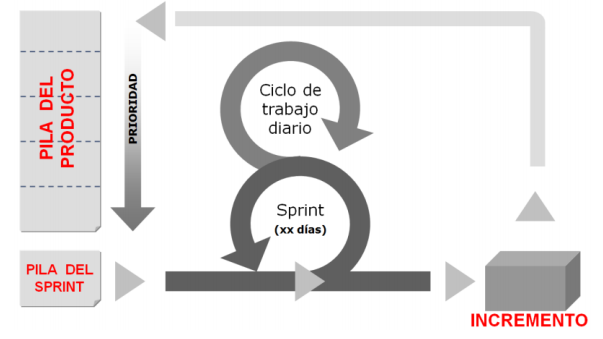
\includegraphics[width=\linewidth]{scrum.png}
  \caption{Diagrama del ciclo iterativo scrum}
  \label{fig:scrum}
\end{figure}

El marco técnico de scrum, \cite{scrum2016} está formado por un conjunto de prácticas y reglas que dan respuesta a los siguientes principios de desarrollo ágil:
\begin{itemize}
	\item Gestión evolutiva del producto, en lugar de la tradicional o predictiva.
	\item Calidad del resultado basado en el \textbf{conocimiento tácito de las personas}, antes que en el explícito de los procesos y la tecnología empleada.
	\item Estrategia de \textbf{desarrollo incremental} a través de iteraciones (sprints).
\end{itemize}

Con la visión general del proyecto, y a partir de ella se especifica y da detalle a las funcionalidades que se desean obtener en primer lugar. Cada ciclo de desarrollo o iteración (\textbf{sprint}) finaliza con la entrega de una parte operativa del producto (\textbf{incremento}). La duración de cada sprint ha sido entre una semana y dos meses.\\

Para diseñar el modelo de datos y la documentación se empleará UML (Lenguaje Unificado de Modelado) y un paradigma de programación OO (Orientado a Objetos). Además se buscará usar una arquitectura MVC (Modelo Vista Controlador) y tener cada parte lo más independiente posible del resto. Esta elección podrá permitir además una mejor integración entre todos los componentes y una mayor facilidad de mantenimiento y ampliación en el futuro.

\section{Planificación del proyecto}
En primer lugar, se realiza una planificación inicial y una investigación sobre las directrices que marca Barbara Kitchenham para crear una revisión sistemática de la literatura sobre un área determinada. Dentro de esta planificación inicial se comprueba que es necesario realizar un sistema de gestión para las distintas revisiones sistemáticas de un usuario, así como un sistema de búsquedas de referencias bibliográficas que pueda sincronizar toda la información con el gestor de referencias Mendeley, y, finalmente, su posterior clasificación según los criterios indicados por el usuario y la exportación de conclusiones finales.\\

Una vez realizada la planificación inicial y analizado todos los objetivos principales del proyecto se decide realizar el desarrollo del proyecto en dos subproyectos. El primero de ellos, será la aplicación web, donde el usuario podrá acceder a todas las opciones para las creaciones de las revisiones sistemáticas de la literatura. Por otro lado, el segundo de ellos consistirá en la creación de una librería JAR donde incluirá todo el proceso de búsquedas de referencias bibliográficas en segundo plano y de manera paralela a cualquier otra búsqueda que se realice. Esta librería, deberá ser incluida en el primer subproyecto, por lo que necesitará de un periodo de tiempo para integrar ambas aplicaciones.\\

Con toda esta información, se opta por dividir el roceso en ocho hitos tal y como podemos ver en la tabla \ref{table:hitos}. El tiempo se indica en dias. Cada uno de estos hitos, tendrá asociados varias subtareas o subobjetivos que deberán realizarse para dar por bueno el hito principal. El hito 0 corresponderá a la adquisición de conocimientos mientras que el hito 7 es asignado a la redacción de la memoria.\\

\begin{table}[!hbt]
	\begin{center}
		\begin{tabular}{|p{2cm}|p{6cm}|p{2.5cm}|p{2.5cm}|}
			\hline
			\textbf{Sprint} & \textbf{Descripción} & \textbf{Estimado} & \textbf{Real}\\
			\hline
			Hito 0 & Propuesta inicial del proyecto & 7 & 5\\
			\hline
			Hito 1 & Investigación y adquisición de conocimientos & 50 & 63\\
			\hline
			Hito 2 & Desarrollo Aplicación Web & 110 & 160\\
			\hline
			Hito 3 & Desarrollo Aplicación Mendeley-REST en Java & 60 & 100\\
			\hline
			Hito 4 & Integración de aplicaciones & 30 & 26\\
			\hline
			Hito 5 & Pruebas del sistema y rendimiento & 10 & 5\\
			\hline
			Hito 6 & Despliegue de la aplicación & 20 & 25\\
			\hline
			Hito 7 & Redacción de memoria & 180 & 280\\
			\hline
		\end{tabular}
		\caption{Tiempo estimado frente a tiempo real de cada Sprint}
		\label{table:hitos}
	\end{center}
\end{table}

Para mostrar el desarrollo detallado de toda la aplicación y desarrollo del software se muestran en las figuras \ref{fig:gantt01}, \ref{fig:gantt02}, \ref{fig:gantt03}, \ref{fig:gantt04} y \ref{fig:gantt05} unos diagramas de Gantt ordenados cronológicamente haciendo referencia a cada uno de los hitos que hemos explicado anteriormente. Los diagramas han sido realizados con la herramienta GanttProject \cite{gantt15}. Cabe indicar, que el hito de mayor duración es el último, que corresponde a la redacción de la documentación de este proyecto, ya que se ha ido redactando a medida que se ha ido completando cada una de las fases del proyecto.\\

\begin{figure}[h!]
	\begin{center}
		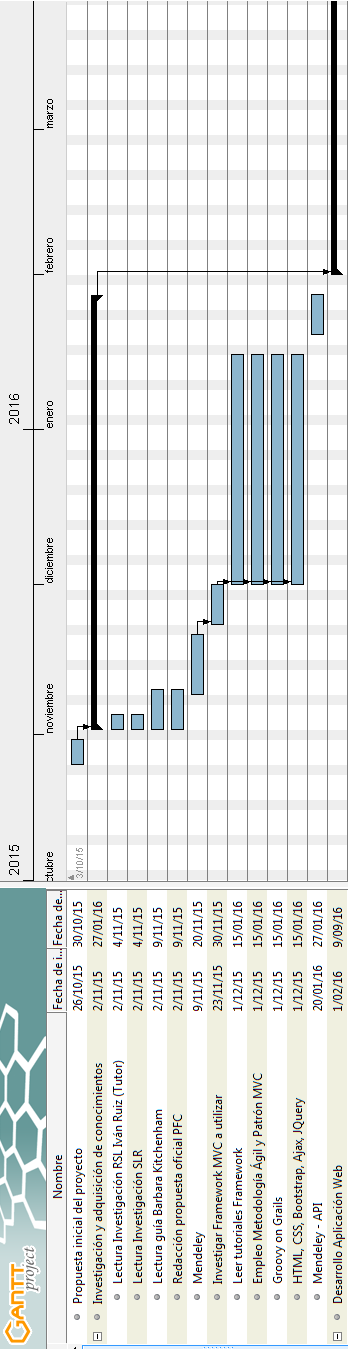
\includegraphics[width=10cm, height=20cm]{gant01.png}
		\caption{Diagrama de Gantt con la propuesta inicial y la adquisición de conocimientos.}
		\label{fig:gantt01}
	\end{center}
\end{figure}

\begin{figure}[h!]
	\begin{center}
		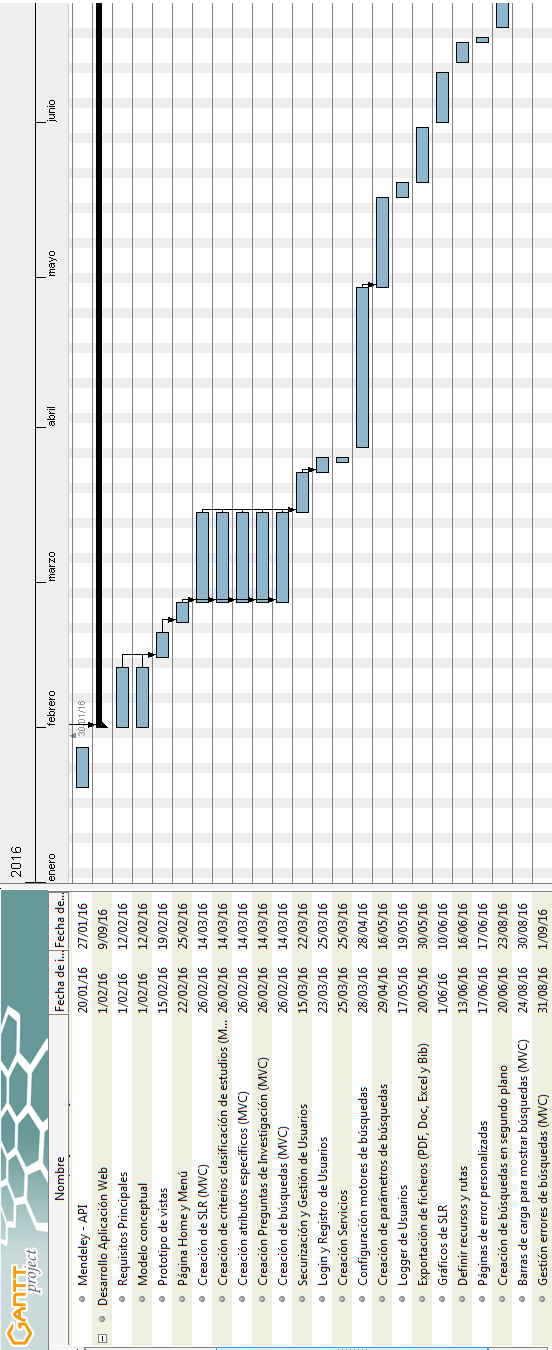
\includegraphics[width=10cm, height=20cm]{gant02.png}
		\caption{Diagrama de Gantt con el Desarrollo de la Aplicación Web.}
		\label{fig:gantt02}
	\end{center}
\end{figure}

\begin{figure}[h!]
	\begin{center}
		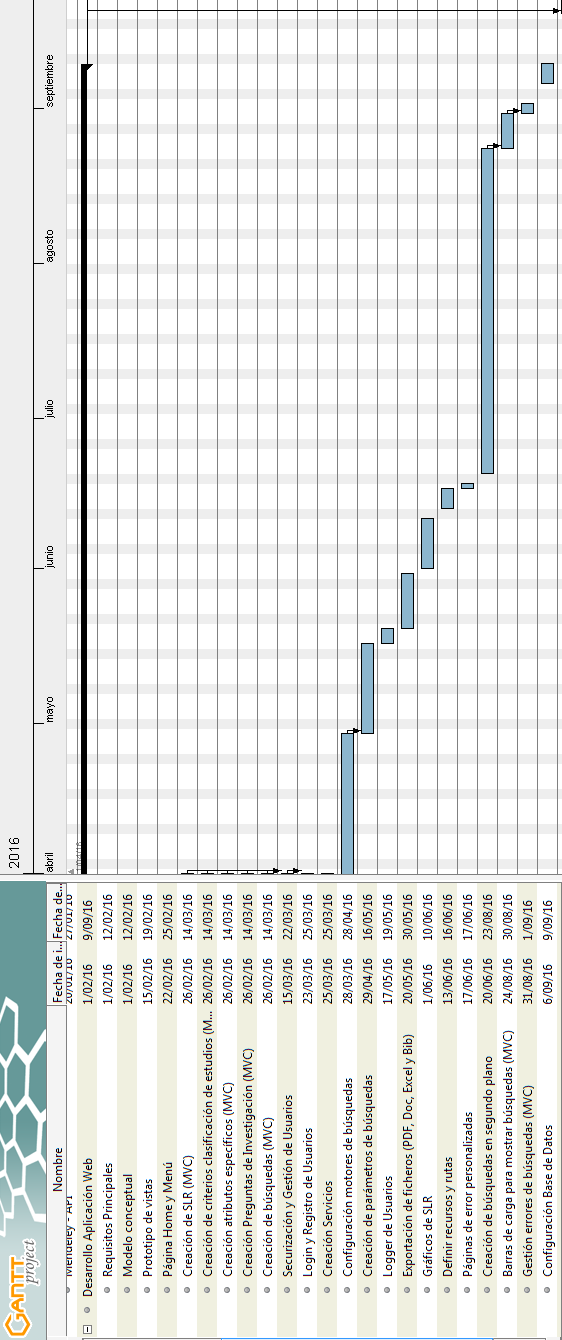
\includegraphics[width=10cm, height=20cm]{gant03.png}
		\caption{Diagrama de Gantt con el Desarrollo de la Aplicación Web (II).}
		\label{fig:gantt03}
	\end{center}
\end{figure}

\begin{figure}[h!]
	\begin{center}
		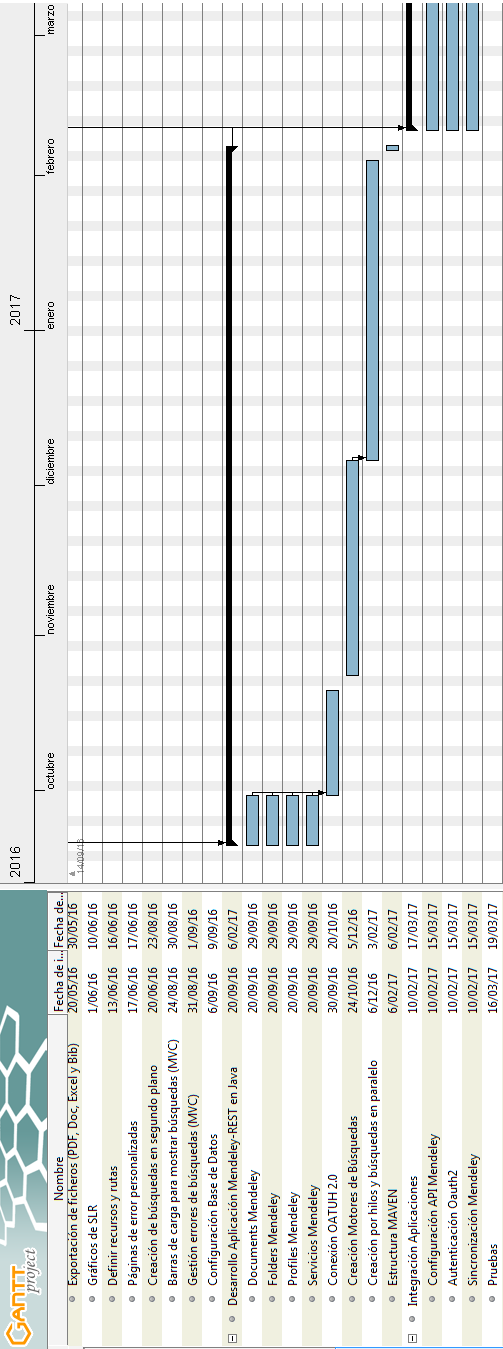
\includegraphics[width=10cm, height=20cm]{gant04.png}
		\caption{Diagrama de Gantt con el Desarroll de la Aplicación Mendeley-REST en Java.}
		\label{fig:gantt04}
	\end{center}
\end{figure}

\begin{figure}[h!]
	\begin{center}
		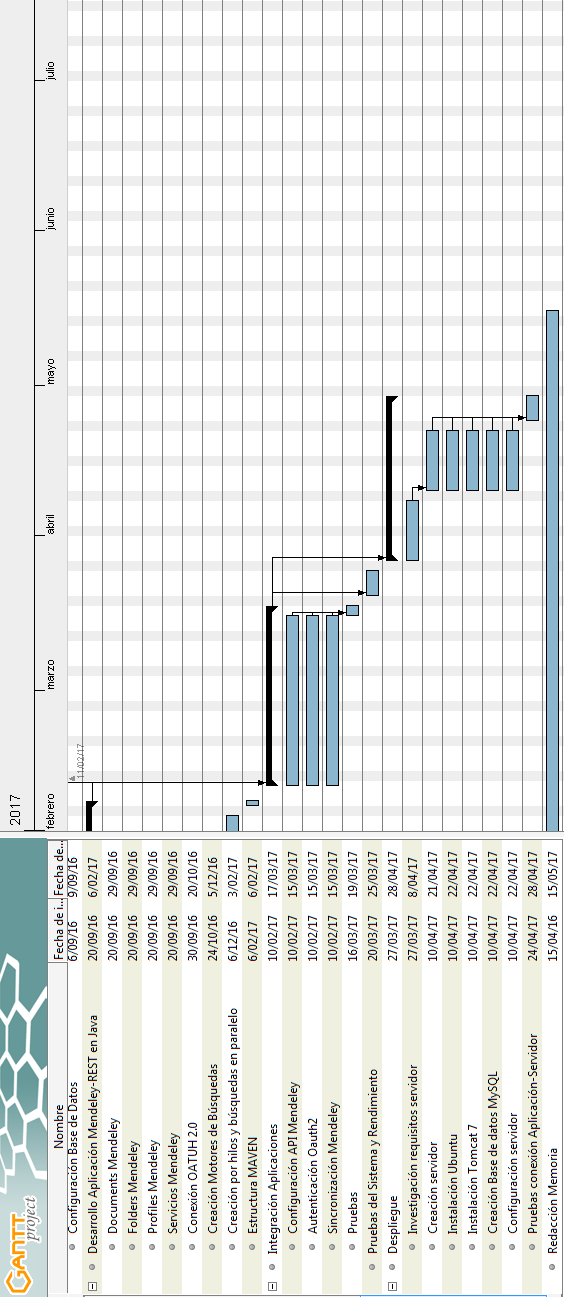
\includegraphics[width=10cm, height=20cm]{gant05.png}
		\caption{Diagrama de Gantt con la Integración de Aplicaciones, Despliegue y Redacción de la memoria.}
		\label{fig:gantt05}
	\end{center}
\end{figure}

%Estimación temporal y definición del calendario básico (hitos principales e iteraciones). Desarrollo de la planificación detallada, utilizando un diagrama de Gantt. Los diagramas de Gantt que se vean correctamente (girados y divididos si hace falta).\\

%Se debe incluir una comparación cuantitativa del tiempo y el esfuerzo realmente invertido frente al estimado y planificado. Estos datos pueden recogerse del sistema de gestión de tareas empleado para el seguimiento del proyecto.



\section{Organización}
En este apartado recogemos las personas o roles que se encuentran involucrados en el proyecto así como una relación de los recursos inventariables utilizados en el proyecto: equipamiento informático, herramientas empleadas, etc.

\subsection{Roles}
En los proyectos que siguen una metodología ágil por SCRUM podemos encontrarnos con tres tipos de roles \cite{scrum2016}:

\begin{itemize}
	\item \textbf{Dueño del producto.} Es el representante del cliente, el cuál conoce el entorno de negocio del cliente, las necesidades y el objetivo que se persigue con el sistema que se construye. Tiene la visión del producto, así como las necesidades concretas del proyecto, para poder priorizar eficientemente el trabajo. El tutor de este proyecto es el más claro ejemplo de representante, así como la UCA ejerce de cliente.
	\item \textbf{Equipo de desarrollo.} Grupo o grupos de trabajo que desarrollan el producto. Todos conocen y comprenden la visión del proprietario del producto. Además, aportan y colaboran con el proprietario en el desarrolo de la pila del producto. En este proyecto el equipo está compuesto únicamente por el autor.
	\item \textbf{Scrum master.} Es el responsable del cumplimiento de las reglas de un marco de scrum técnico, asegurando que se entienden en la organización, y se trabaja confirme a ellas. Además, proporciona la asesoría y formación necesaria al proprietario del producto y al equipo. En el proyecto estará representado por el autor, por lo que éste representará tanto al equipo de desarrollo como al scrum master.
\end{itemize}

\subsection{Recursos}
En este apartado se van a listar todos los recursos inventariables de hardware y software, así como las herramientas utilizadas y los lenguajes de programación.\\

En primer lugar se listan los recursos de hardware.\\

\begin{itemize}
	\item Equipo donde se ha realizado el proyecto: Toshiba Satellite L750/L755, Intel  \textregistered Core \texttrademark  i5-2410M CPU @ 2.30GHz x 2, 4GB RAM
	\item Servidor donde se ha desplegado el proyecto: 1 vCore CPU, 2048MB RAM, 40 GB SSD Storage, 2000 GB Bandwitch
\end{itemize}

A continuación se listan los recursos de software
\begin{itemize}
	\item Equipo donde se ha realizado el proyecto:
	
	\begin{itemize}
		\item SO: Windows 7 64 bits
		\item API Externa: Google Charts y Mendeley
	\end{itemize}
	
	\item Servidor donde se ha desplegado el proyecto:
	
	\begin{itemize}
		\item SO: Ubuntu 16.04 7 64 bits
		\item Contenedor Web: Tomcat 7 64 bits
		\item Base de Datos: MySql
	\end{itemize}
\end{itemize}

A continuación se listan las herramientas empleadas.\\
\begin{itemize}
	\item IDE: Grails Tool Suite
	\item Control de versiones: Subversion
	\item Forja: Assembla
	\item SGBD: Mysql
	\item Diseño de diagramas: DIA
	\item Diseño de Mockups: Balsamiq Mockups
	\item Navegadores empleados: Firefox y Google Chrome
	\item Memoria y presentación: \LaTeX
	\item Procesador de texto: Microsoft Word 2010
	\item Gestión Hojas de cálculo: Microsoft Excel 2010
	\item Vision de documentos: Adobe Acrobat Reader
\end{itemize}

Para finalizar, se listan los lenguajes de programación utilizados:\\
\begin{itemize}
	\item Groovy
	\item Java
	\item JavaScript
	\item Ajax
	\item JQuery
	\item CSS3
	\item Bootstrap
	\item HTML
\end{itemize}

\section{Costes}
Para poder realizar una estimación de los costes del proyecto debemos tener en cuenta tanto los recursos humanos como los recursos en material empleados. Los costes indirectos como papel, bolígrafo, electricidad o conexión a Internet son los que denominaremos ``Costes indirectos``. El porcentaje de su valor puede oscilar entre el 10\% y el 20\% del gasto del personal, tomaremos el gasto medio de dicho intervalo, es decir, un 15\%.\\

De los recursos hardware debemos tener en cuenta tanto el equipo empleado para el desarrollo. Normalmente, los ordenadores suelen tener un periodo de amortización entre los 2 y 4 años. Al igual que antes, tomaremos la media de este periodo, 3 años. Si el equipo costó 750 euros, se amortizan unos 250 euros al año y como el tiempo de desarrollo del proyecto es de entre 2 y 3 años a tiempo parcial, tomaremos 2,5 años como periodo medio y el coste final será de 625 euros. El coste del servidor son de unos 10 euros al mes, sólamente ha estado desplegado en el servidor alrededor de 3 meses, por lo que su gasto alcanza los 30 euros.\\

Con respecto a los recursos del software, no tendrá ningún gasto, puesto que el sistema operativo Windows 7 viene incluido en los gastos del equipo con el que se ha desarrollado el proyecto, así como los paquetes informáticos (hojas de cálculo y editor de texto). Además, el servidor tiene instalado Ubuntu y tampoco supone ningún gasto económico puesto que viene en el gasto mensual del servidor.\\

Para el cálculo de costes de personal se ha consultado las tablas salariales de la UCA para el personal técnico de apoyo contratado laboral \cite{paslaboral}. El coste es de unos 20.298,30 euros anuales, lo equivale a 1.353,22 euros mensuales. Como el tiempo dedicado en este tiempo ha sido lo correspondiente a media jornada, tomaremos como un gasto mensual de 676.61 euros. De esta manera, el coste anual será de unos 8119.32 euros y alcanzaremos unos gastos anuales de 20298 euros.\\

En la tabla \ref{table:costes} desglosamos los costes mensuales y totales del proyecto:

\begin{table}[!hbt]
	\begin{center}
		\begin{tabular}{|p{2cm}|p{6cm}|p{2.5cm}|p{2.5cm}|}
			\hline
			\textbf{Unidades} & \textbf{Descripción} & \textbf{Coste Unitario} & \textbf{Coste total}\\
			\hline
			1 & Ingeniero Técnico Informático & 8119.32 \euro/año & 20298 \euro\\
			\hline
			1 & Ordenador personal & 286.67 \euro/año & 625 \euro\\
			\hline
			1 & Alquiler Host & 10 \euro/mes & 30 \euro\\
			\hline
			1 & Costes indirectos & 1217 \euro/año & 3044 \euro\\
			\hline
			\multicolumn{3}{|c|}{\textbf{Total}} & 23967 \euro\\
			\hline
		\end{tabular}
		\caption{Costes del desarrollo}
		\label{table:costes}
	\end{center}
\end{table}

%Estudio y presupuesto de los costes de los recursos (humanos y materiales) descritos anteriormente, necesarios para el proyecto.

%Para el cálculo de costes de personal pueden consultarse las tablas salariales de la UCA para el personal técnico de apoyo contratado laboral \cite{paslaboral}, o bien otras más ajustadas a la realidad. El cálculo del coste del personal del proyecto debe hacerse en personas-mes, y luego hacer la correspondencia al coste monetario.\\

\section{Riesgos}
En esta sección vamos a describir los posibles riesgos del proyecto ordenados de mayor a menor prioridad, indicando su posible impacto (efecto que la ocurrencia del citado riesgo tendría en el desarrollo del proyecto) y la probabilidad de ocurrencia. Además, indicamos el plan necesario para reducir los efectos del riesgo una vez se haya materializado o disminuir que este ocurra. Esta información viene recogida en la tabla \ref{table:riesgos}.

\begin{table}[!hbt]
	\begin{center}
		\begin{tabular}{|p{3.5cm}|p{1.5cm}|p{2cm}|p{6cm}|}
			\hline
			\textbf{Riesgo} & \textbf{Prob.} & \textbf{Magnitud} & \textbf{Plan a realizar}\\
			\hline
			Tiempo infraestimado para el desarrollo de las tareas & 30\% & 5-8 semanas & Se comunica al tutor del proyecto del posible retraso, modificando la planificación temporal del proyecto o bien el plazo de entrega para poder finalizarlo.\\
			\hline
			Desarrollo de métodos y funciones software incorrectos & 30\% & 3-4 semanas & Se comprueba la calidad del código y su validez, para así evitar el denominado \textbf{DRY} (\textit{Don't Repeat yourself}) y estudiar su re-utilización una vez corregido.\\
			\hline
			Cambios en API de Mendeley & 30\% & 3 semanas & Comunicar al tutor del proyecto del posible retraso y realizar una rápida investigación de los cambios producidos en la API de Mendeley, así como el desarrollo de la nueva implementación de la misma.\\
			\hline
			Cambios en API de motores de búsquedas de referencias bibliográficas & 30\% & 3 semanas & Comunicar al tutor del proyecto del posible retraso y realizar una rápida investigación de los cambios producidos en los motores de búsquedas, como el desarrollo de la nueva implementación de los mismos.\\
			\hline
			Elección incorrecta en las herramientas empleadas de desarrollo & 15\% & 2-3 semanas & Comunicar al tutor del proyecto del posible retraso y realizar una rápida investigación de las nuevas herramientas a emplear, así como de la búsqueda y lectura de documentación.\\
			\hline
			Paro del proyecto & 20\% & 1-2 semanas & Revisar la planificación y ajustarla, así como añadir horas extras una vez que se retome el desarrollo.\\
			\hline
			Problemas en los tests & 30\% & 1-2 semanas & Se analizan los tests y se planteará la nueva revisión de éstos y, en el caso correspondiente, crear unos nuevos.\\
			\hline
		\end{tabular}
		\caption{Lista de riesgos del proyecto}
		\label{table:riesgos}
	\end{center}
\end{table}

%Enumeración de los riesgos del proyecto, indicando su posible impacto (efecto que la ocurrencia del citado riesgo tendría en el desarrollo del proyecto) y la probabilidad de ocurrencia. Una vez los riesgos son identificados y priorizados, hay que definir los planes necesarios para reducir los efectos del riesgo una vez se haya materializado o disminuir que este ocurra.\\

\section{Aseguramiento de calidad}
Para asegurar el cumplimiento de la calidad de este se contempla los siguientes aspectos:\\

\begin{itemize}
	\item Realización de controles o pruebas para asegurar su calidad.
	\item Tomar medidas de actuación relacionadas con el control de calidad.
\end{itemize}

Se realizará un análisis para cada uno de los hitos o tareas, con lo que es necesario un plan de verificación y validación dentro de los mismos para poder asegurar la calidad del producto y el correcto funcionamiento de los mismos. Estas comprobaciones se realizarán a lo largo del proyecto y así comprobar que todo está correcto y se cumple los requisitos establecidos.\\

%En esta sección se incluirán las actividades y tareas relacionadas con el aseguramiento de calidad a realizar durante el desarrollo del software. Se incluirán los estándares, prácticas y normas aplicables durante el desarrollo del software.\\

%También, deberán recogerse los diferentes tipos de revisiones, verificaciones y validaciones que se van a llevar a cabo, los criterios para la aceptación o rechazo de cada producto y los procedimientos para implementar acciones correctoras o preventivas.


% DESARROLLO
\part{Desarrollo}
%\null\vfill
%\noindent En esta parte se debe describir el desarrollo del proyecto siguiendo la metodología empleada. Sus capítulos no deben ser una descripción exhaustiva de todos los documentos, diagramas, código fuente y, en general, entregables generados, sino más bien una explicación resumida del desarrollo, estructurada según las etapas principales del proceso de ingeniería. Deben seleccionarse aquellos diagramas, fragmentos de código y secciones de los entregables que sean más significativos para dicha explicación. La totalidad de los entregables resultado del proyecto se ubicarán en los anexos y/o en el material en CD/DVD que acompañe al proyecto.

\chapter{Requisitos del Sistema}
\label{chap:chap03}
% ------------------------------------------------------------------------------
% Este fichero es parte de la plantilla LaTeX para la realización de Proyectos
% Final de Grado, protegido bajo los términos de la licencia GFDL.
% Para más información, la licencia completa viene incluida en el
% fichero fdl-1.3.tex

% Copyright (C) 2012 SPI-FM. Universidad de Cádiz
% ------------------------------------------------------------------------------

En esta sección se detalla la situación actual de la organización y las necesidades de la misma, que originan el desarrollo o mejora de un sistema informático. Luego se presentan los objetivos y el catálogo de requisitos del nuevo sistema. Finalmente se describen las diferentes alternativas tecnológicas y el análisis de la brecha entre los requisitos planteados y la solución base seleccionada, si aplica.

%\section{Situación actual} 
%Esta sección debe contener información sobre la situación actual de la organización para la que se va a desarrollar el sistema software.

%\subsection{Procesos de Negocio}
%Esta sección debe contener información sobre los modelos de procesos de negocio actuales, que suelen ser la base de los modelos de procesos de negocio a implantar.

%\subsection{Entorno Tecnológico}
%Esta sección debe contener información general sobre el entorno tecnológico en la organización del cliente antes del comienzo del desarrollo del sistema software, incluyendo hardware, redes, software, etc.

%\subsection{Fortalezas y Debilidades}
%Esta sección debe contener información sobre los aspectos positivos y negativos del negocio actual de la organización para la que se va a desarrollar el sistema software.

\section{Necesidades de Negocio}
%Esta sección debe contener información sobre los objetivos de negocio de clientes y usuarios, incluyendo los modelos de procesos de negocio a implantar.
Este apartado contendrá información sobre los objetivos de negocio tanto del cliente como de los usuarios, incluyendo los models de procesos de negocio a implantar.

\subsection{Objetivos de Negocio}
%Esta sección debe contener los objetivos de negocio que se esperan alcanzar cuando el sistema software a desarrollar esté en producción.
El objetivo principal es la realización de una aplicación web con la que un usuario pueda automatizar, en la mayor parte posible, todas las etapas de creación de revisiones sistemáticas de la literatura.\\

Una vez que el cliente tome la decisión de realizar una determinada investigación, deberá de realizar la búsqueda de la literatura que precisa para extraer conclusiones al final del mismo. Por ello, necesita un sistema con el que realizar varias búsquedas sobre varios motores de referencias específicos a la vez con las que posteriormente, el cliente estudiará, clasificará y exportará dicha información para obtener las conclusiones finales.\\

\subsection{Procesos de Negocio}
%Esta sección, debe contener los modelos de procesos de negocio a implantar, que normalmente son los modelos de procesos de negocio actuales con ciertas mejoras.
Este punto queda fuera del ámbito del proyecto, ya que no se implantará ningún modelo de proceso de negocio en esta aplicación. La forma de emplear este producto queda a decisión del cliente o investigador.

\section{Objetivos del Sistema}
Tal y como hemos descrito, el objetivo final de este proyecto es ayudar al investigador a automatizar algunas de las fases de las revisiones sistemáticas de la literatura.\\

Para ello, el autor de una revisión sistemática, deberá seguir todas y cada una de las fases y la aplicación web ofrecerá todas las herramientas posibles para extraer la literatura deseada, así como la clasificación de qué estudios son válidos y cuáles no y, por último, la exportación de los datos en varios formatos de ficheros o la visualización de gráficas que ayuden a determinar las conclusiones finales del estudio.\\

\section{Catálogo de Requisitos}
%Esta sección debe contener la descripción del conjunto de requisitos específicos del sistema a desarrollar para satisfacer las necesidades de negocio del cliente.
A continuación vamos a detallar el conjunto de requisitos específicos del sistema a desarrollar y con el que se pretende satisfacer las necesidades del cliente.

\subsection{Requisitos funcionales}
%Descripción completa de la funcionalidad que ofrece el sistema. 
Los requisitos funcionales que ofrece el sistema estarán separados en dos grupos, dependiendo de si estamos hablando de un cliente que además, tenga permisos de administrador (Rol Administrador) o no (Rol Usuario).

\begin{itemize}
	\item \textbf{Rol Usuario}
		\begin{itemize}
			\item Creación de revisiones sistemáticas de la literatura
			\item Realizar búsquedas de referencias bibliográficas para los SLR.
			\item Clasificar las referencias bibliográficas por medio de criterios de clasificación aportados por el usuario.
			\item Obtener información de las referencias bibliográficas, así como la posibilidad de insertar nuevos campos o metadatos sobre los mismo.
			\item Exportar la información obtenida del estudio de la investigación a través de varios formatos de salida.
			\item Visualizar gráficos con la información obtenida de todas las búsquedas.
	\end{itemize}
	\item \textbf{Rol Administrador}
	
	\begin{itemize}
		\item Todas las tareas del Rol Usuario.
		\item Gestión de usuarios del sistema.
		\item Gestión de errores en procesos de búsquedas.
		\item Gestión de motores de búsquedas de referencias bibliográficas.
		\item Gestión API REST de Mendeley con la aplicación.
	\end{itemize}
\end{itemize}

\subsection{Requisitos no funcionales}
%Descripción de otros requisitos (relacionados con la calidad del software) que el sistema deberá satisfacer: portabilidad, seguridad, estándares de obligado cumplimiento, accesibilidad, usabilidad, etc.
Descripción de otros requisitos que el sistema deberá satisfacer:

\begin{itemize}
	\item Todos los módulos de la aplicación web deberán estar disponibles para su instalación por parte de la UCA. Para ello, se ha decidido subir todo la aplicación en un repositorio al que puedan acceder.
	\item La aplicación deberá tener un alto grado de accesibilidad y usabilidad, ya que se espera que en el futuro haya personas que puedan acceder y modificar o mejorar cualquier componente del sistema.
	\item El sistema deberá ser seguro, las revisiones sistemáticas de cada usuario tienen acceso restringido a cualquier otro a no ser que tenga permisos para hacerlo.
	\item El sistema deberá ser portable en cualquiera de los navegadores web.
	\item El proceso de búsqueda de referencias deberá ser lo más transparente posible al usuario.
\end{itemize}

\subsection{Reglas de negocio}
%En el desarrollo del sistema, hay que tener en cuenta las denominadas reglas de negocio, es decir, el conjunto de restricciones, normas o políticas de la organización que deben ser respetadas por el sistema, las cuales suelen ser cambiantes.
Para el desarrollo del sistema, se ha indicado las siguientes reglas de negocio:

\begin{itemize}
	\item La aplicación web deberá ser desarrollado bajo un framework que permita utilizar el patrón \textbf{MVC} (\textit{Model View Controller}) para permitir la implementación de módulos independientes en el sistema si se desea.
	\item El usuario debe estar registrado en Mendeley. De esta manera, el usuario dispondrá de un gestor de referencias donde la aplicación web insertará toda la documentación que la aplicación web encuentre.
	\item La aplicación debe permitir la posibilidad de insertar un nuevo motor de búsqueda, para ello se explicará más adelante como un usuario administrador del sistema puede descargar el código de la aplicación e insertarlo.
\end{itemize}

\subsection{Requisitos de información}
%En esta sección se describen los requisitos de gestión de información (datos) que el sistema debe gestionar.
Describimos a los requisitos de gestión de información (datos) que el sistema debe gestionar en las tablas \ref{table:irq01}, \ref{table:irq02}, \ref{table:irq03}, \ref{table:irq04}, \ref{table:irq05}, \ref{table:irq06}, \ref{table:irq07} y \ref{table:irq08}.

\begin{table}[!hbt]
	\begin{center}
		\begin{tabular}{|p{5cm}|p{10cm}|}
			\hline
			\textbf{IRQ-01} & Información de usuarios.\\
			\hline
			\textbf{Objetivos asociados} & OBJ-01 \ref{table:obj01}\\
			\hline
			\textbf{Requisitos asociados} & -\\
			\hline
			\textbf{Datos específicos} & \shortstack[l]{Email Mendeley \\ Password Mendeley \\ Rol} \\
			\hline
			\textbf{Estabilidad} & Alta\\
			\hline
			\textbf{Comentarios} & Información de los usuarios para hacer login con Mendeley.\\
			\hline
		\end{tabular}
		\caption{IRQ-01: Requisitos de información de los usuarios.}
		\label{table:irq01}
	\end{center}
\end{table}

\begin{table}[!hbt]
	\begin{center}
		\begin{tabular}{|p{5cm}|p{10cm}|}
			\hline
			\textbf{IRQ-02} & Información de revisiones sistemáticas de la literatura.\\
			\hline
			\textbf{Objetivos asociados} & OBJ-01 \ref{table:obj01}\\
			\hline
			\textbf{Requisitos asociados} & -\\
			\hline
			\textbf{Datos específicos} & \shortstack[l]{Identificador \\ Título \\ Justificación} \\
			\hline
			\textbf{Estabilidad} & Alta\\
			\hline
			\textbf{Comentarios} & Información de las revisiones sistemáticas de la literatura.\\
			\hline
		\end{tabular}
		\caption{IRQ-02: Requisitos de información de las revisiones sistemáticas de la literatura.}
		\label{table:irq02}
	\end{center}
\end{table}

\begin{table}[!hbt]
	\begin{center}
		\begin{tabular}{|p{5cm}|p{10cm}|}
			\hline
			\textbf{IRQ-03} & Información de las búsquedas de referencias bibliográficas de un SLR.\\
			\hline
			\textbf{Objetivos asociados} & OBJ-02 \ref{table:obj02}\\
			\hline
			\textbf{Requisitos asociados} & -\\
			\hline
			\textbf{Datos específicos} & \shortstack[l]{Identificador \\ Términos búsqueda \\ Motores Búsquedas \\ Total referencias a buscar \\ Rango años} \\
			\hline
			\textbf{Estabilidad} & Alta\\
			\hline
			\textbf{Comentarios} & Información de las búsquedas de referencias bibliográficas de un SLR.\\
			\hline
		\end{tabular}
		\caption{IRQ-03: Requisitos de información de las búsquedas de referencias bibliográficas de un SLR.}
		\label{table:irq03}
	\end{center}
\end{table}

\begin{table}[!hbt]
	\begin{center}
		\begin{tabular}{|p{5cm}|p{10cm}|}
			\hline
			\textbf{IRQ-04} & Información de las referencias bibliográficas de un SLR.\\
			\hline
			\textbf{Objetivos asociados} & OBJ-01 \ref{table:obj01} y OBJ-02 \ref{table:obj02}\\
			\hline
			\textbf{Requisitos asociados} & IRQ-03 \ref{table:irq03}\\
			\hline
			\textbf{Datos específicos} & \shortstack[l]{Identificador \\ Título \\ Autores \\ Publicación \\ Año publicación \\ Idioma \\ Abstract \\ Palabras clave \\ enlaces de referencia \\ Páginas \\ Volumen \\ Criterio} \\
			\hline
			\textbf{Estabilidad} & Alta\\
			\hline
			\textbf{Comentarios} & Información de las referencias bibliográficas de un SLR.\\
			\hline
		\end{tabular}
		\caption{IRQ-04: Requisitos de información de las referencias bibliográficas de un SLR.}
		\label{table:irq04}
	\end{center}
\end{table}

\begin{table}[!hbt]
	\begin{center}
		\begin{tabular}{|p{5cm}|p{10cm}|}
			\hline
			\textbf{IRQ-05} & Información de criterios de clasificación de un SLR.\\
			\hline
			\textbf{Objetivos asociados} & OBJ-01 \ref{table:obj01}, OBJ-02 \ref{table:obj02} y OBJ-03 \ref{table:obj03}\\
			\hline
			\textbf{Requisitos asociados} & IRQ-03 \ref{table:irq03} y IRQ-04 \ref{table:irq04} \\
			\hline
			\textbf{Datos específicos} & \shortstack[l]{Identificador \\ Nombre \\ Total referencias} \\
			\hline
			\textbf{Estabilidad} & Alta\\
			\hline
			\textbf{Comentarios} & Información de los criterios de clasificación de una revisión sistemática de la literatura.\\
			\hline
		\end{tabular}
		\caption{IRQ-05: Requisitos de información de los criterios de clasificación de un SLR.}
		\label{table:irq05}
	\end{center}
\end{table}

\begin{table}[!hbt]
	\begin{center}
		\begin{tabular}{|p{5cm}|p{10cm}|}
			\hline
			\textbf{IRQ-06} & Información de preguntas de investigación de un SLR.\\
			\hline
			\textbf{Objetivos asociados} & OBJ-01 \ref{table:obj01}\\
			\hline
			\textbf{Requisitos asociados} & IRQ-02 \ref{table:irq02}\\
			\hline
			\textbf{Datos específicos} & \shortstack[l]{Identificador \\ Enunciado} \\
			\hline
			\textbf{Estabilidad} & Alta\\
			\hline
			\textbf{Comentarios} & Información de las preguntas de investigación asociadas a una revisión sistemática de la literatura.\\
			\hline
		\end{tabular}
		\caption{IRQ-06: Requisitos de información de las preguntas de investigación de un SLR.}
		\label{table:irq06}
	\end{center}
\end{table}

\begin{table}[!hbt]
	\begin{center}
		\begin{tabular}{|p{5cm}|p{10cm}|}
			\hline
			\textbf{IRQ-07} & Información de metadatos específicos de una referencia en un SLR\\
			\hline
			\textbf{Objetivos asociados} & OBJ-02 \ref{table:obj02} y OBJ-03 \ref{table:obj03}\\
			\hline
			\textbf{Requisitos asociados} & IRQ-03 \ref{table:irq03} y IRQ-04 \ref{table:irq04}\\
			\hline
			\textbf{Datos específicos} & \shortstack[l]{Identificador \\ Nombre \\ Tipo Campo \\ Valor defecto} \\
			\hline
			\textbf{Estabilidad} & Alta\\
			\hline
			\textbf{Comentarios} & Información de los metadatos específicos de una referencia en un SLR.\\
			\hline
		\end{tabular}
		\caption{IRQ-07: Requisitos de información de los metadatos específicos de una referencia en un SLR.}
		\label{table:irq07}
	\end{center}
\end{table}

\begin{table}[!hbt]
	\begin{center}
		\begin{tabular}{|p{5cm}|p{10cm}|}
			\hline
			\textbf{IRQ-08} & Información de información a exportar de un SLR\\
			\hline
			\textbf{Objetivos asociados} & OBJ-02 \ref{table:obj02} y OBJ-04 \ref{table:obj04}\\
			\hline
			\textbf{Requisitos asociados} & IRQ-02 \ref{table:irq02}, IRQ-03 \ref{table:irq03}, IRQ-04 \ref{table:irq04}, IRQ-05 \ref{table:irq05}, IRQ-06 \ref{table:irq05} y IRQ-07 \ref{table:irq07} \\
			\hline
			\textbf{Datos específicos} & \shortstack[l]{Datos SLR \\ Datos Búsquedas \\ Datos referencias} \\
			\hline
			\textbf{Estabilidad} & Alta\\
			\hline
			\textbf{Comentarios} & Información a exportar de un SLR.\\
			\hline
		\end{tabular}
		\caption{IRQ-08: Requisitos de información de los datos a exportar de un SLR.}
		\label{table:irq08}
	\end{center}
\end{table}

\section{Alternativas de Solución}
%En esta sección, se debe ofrecer un estudio del arte de las diferentes alternativas tecnológicas que permitan satisfacer los requerimientos del sistema, para luego seleccionar (si procede) la herramienta o conjunto de herramientas que utilizaremos como base para el software a desarrollar.
Para el desarrollo de esta aplicación, se pensó en la posibilidad de crear un \textbf{DSL} textual (\textbf{Domain Specific Language}) donde el usuario por línea de comandos escribiera las instrucciones para conectar con el motor de búsqueda de referencias y descargar las referencias encontradas. En la UCA se trabaja con Eclipse como IDE de desarrollo, pero era un entorno complejo para desarrollar DSL debido a la poca documentación que existe en la actualidad. Además, la creación de un SLR sería llevada mejor a cabo si el usuario puede ver en todo momento la realización del mismo así como todos los pasos y directrices necesarios para el proceso.\\

Finalmente, se tomó la decisión de realizar una aplicación web con el que los investigadores tendrán un fácil acceso y de manera visual obtener las conclusiones finales y, además, de un fácil desarrollo y mantenimiento gracias al framework \textit{Groovy on Grails} que nos permite aplicar el patrón \textit{MVC} y realizar un mejor mantenimiento de la aplicación.

\section{Solución Propuesta}
%Si se ha optado por utilizar un software de base, debemos identificar y medir las diferencias entre lo que proporciona este software y los requisitos definidos para el proyecto.\\
%El resultado de este análisis permitirá identificar cuáles de éstos requisitos ya están solventados total o parcialmente por el sistema base y cuales tendremos que diseñar e implementar la propuesta de solución.
El desarrollo propuesto será la realización de un sistema web, donde el usuario podrá conectar a través de su cuenta de Mendeley y crear las revisiones sistemáticas de la literatura que considere necesario.\\

La aplicación al ser en un entorno web, se desarrolla con un IDE denominado \textit{Grails Tool Suite} donde por medio de los lenguajes \textit{Groovy} y \textit{Java} podemos aplicar el patrón MVC y desarrollar una aplicación fácil de mantener y modularizada.\\

Mendeley ofrece un gestor de referencias al usuario por medio de una API REST con la que desde una aplicación, como este proyecto de fin de carrera, pueda conectarse y obtener la información necesaria para realizar los estudios de la literatura y permitir la sincronización de datos entre ambas.\\

\chapter{Análisis del Sistema}
\label{chap:chap04}
% ------------------------------------------------------------------------------
% Este fichero es parte de la plantilla LaTeX para la realización de Proyectos
% Final de Grado, protegido bajo los términos de la licencia GFDL.
% Para más información, la licencia completa viene incluida en el
% fichero fdl-1.3.tex

% Copyright (C) 2012 SPI-FM. Universidad de Cádiz
% ------------------------------------------------------------------------------

Esta sección cubre el análisis del sistema de información a desarrollar, haciendo uso del lenguaje de modelado UML.

\section{Modelo Conceptual}
A partir de los requisitos de información, se desarrollará un diagrama conceptual de clases UML. En ella identificaremos las clases, atributos y relaciones entre ellas tal y como podemos ver en la figura \ref{fig:digclases}.

\begin{figure}[!hpt]
	\begin{center} 
		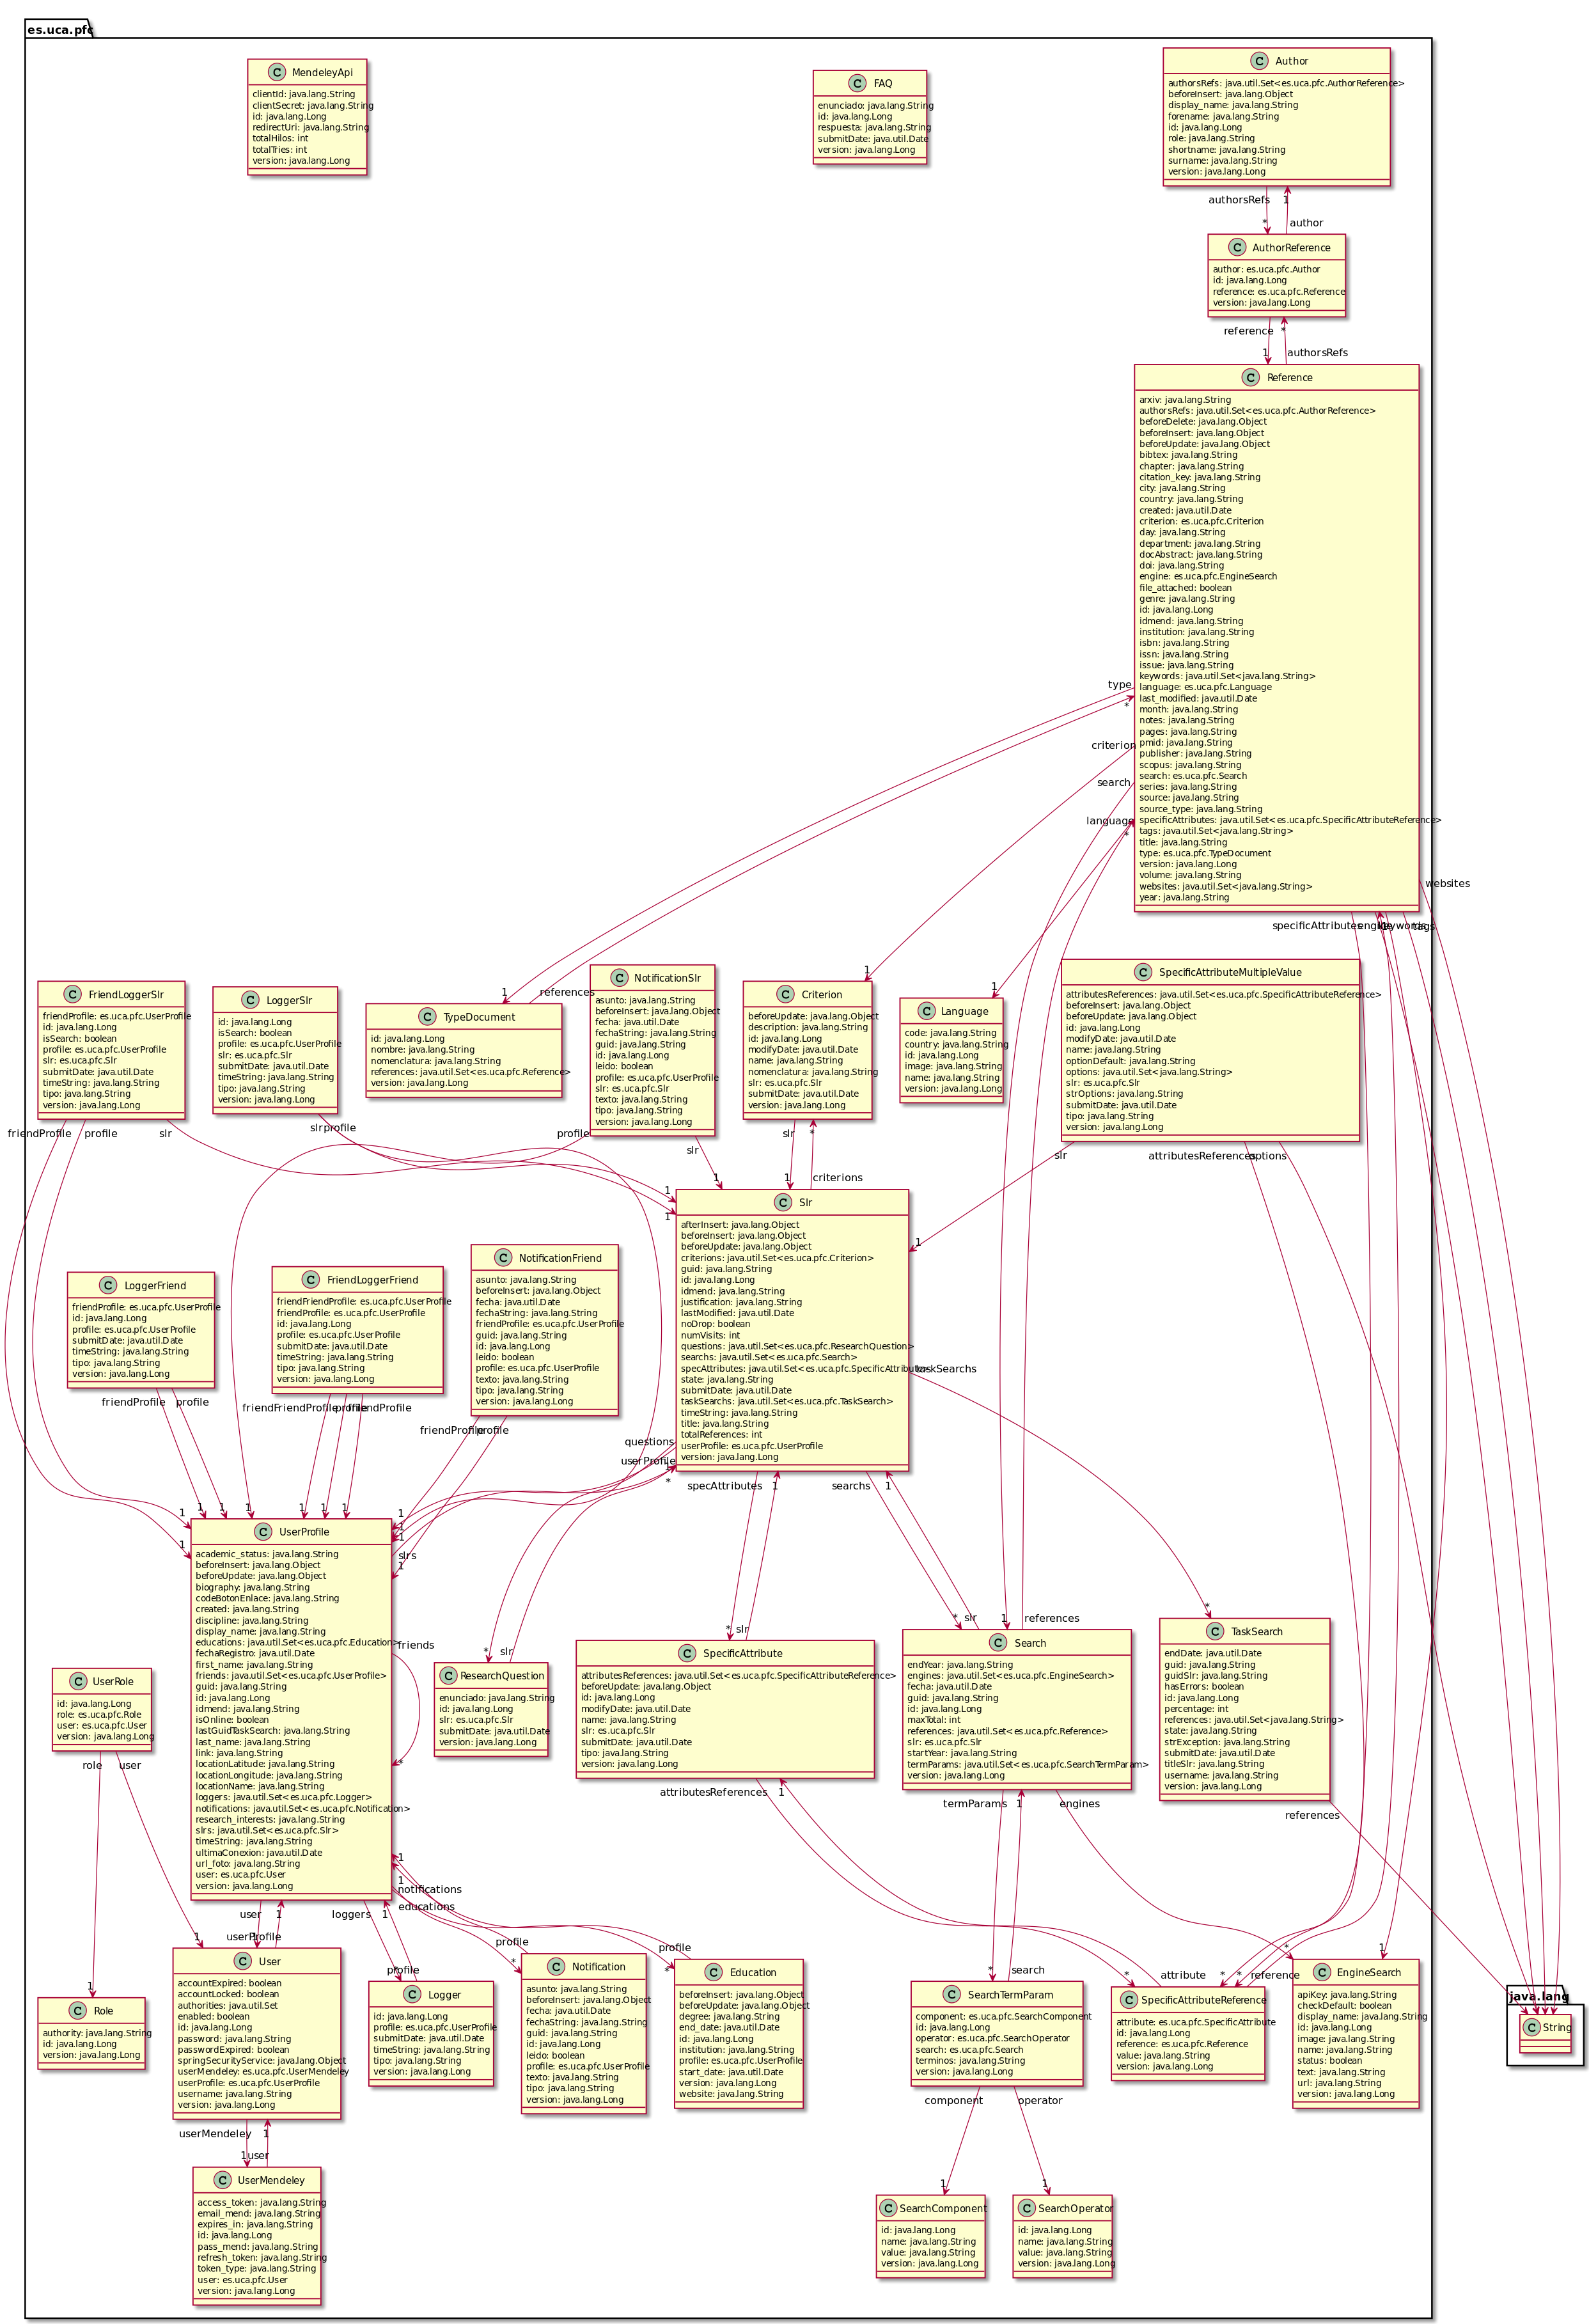
\includegraphics[width=\linewidth]{class-diagram.png}
		\caption{Diagrama conceptual de clases UML.}
		\label{fig:digclases}
	\end{center}
\end{figure}

%A partir de los requisitos de información, se desarrollará un diagrama conceptual de clases UML, identificando las clases, atributos, relaciones, restricciones adicionales y reglas de derivación necesarias.

\section{Modelo de Casos de Uso}
A partir de los requisitos funcionales descritos en apartados anteriores, se emplearan los casos de uso como mecanismo para representar las interacciones entre los actores y el sistema a desarrollar.
%A partir de los requisitos funcionales descritos anteriormente, se emplearan los casos de uso como mecanismo para representar las interacciones entre los actores y el sistema bajo estudio. Para cada caso de uso deberá indicarse los actores implicados, las precondiciones y postcondiciones, los pasos que conforman el escenario principal y el conjunto de posibles escenarios alternativos.

\subsection{Actores} 
Los diferentes roles que con el sistema pueden interactuar son los siguientes:

\begin{itemize}
	\item Investigador. Esta figura representa el usuario principal del sistema web. Una persona con este rol podrá realizar revisiones sistemáticas de la literatura y efectuar todas las tareas relacionadas con ellas.
	\item Administrador. Esta figura podrá realizar todas las funciones del rol investigador, junto con el mantenimiento de gestión de los usuarios y los errores de búsquedas de referencias bibliográficas producidas en el sistema.
\end{itemize}

%En este apartado se describirán los diferentes roles que juegan los usuarios que interactúan con el sistema. Los actores pueden ser roles de personas físicas, sistemas externos o incluso el tiempo (eventos temporales).

\subsection{Diagramas y especificación de casos de uso}
En esta sección se mostrarán los diagramas de casos de uso de la aplicación web (\ref{fig:cu01}, \ref{fig:cu02}, \ref{fig:cu03}, \ref{fig:cu04}, \ref{fig:cu05}, \ref{fig:cu06}, \ref{fig:cu07}, \ref{fig:cu08}), así como la especificación de los mismos mediante escenarios de casos de uso tal y como describimos en las tablas correspondientes a cada caso de uso.

\begin{figure}[hp!]
	\begin{center} 
		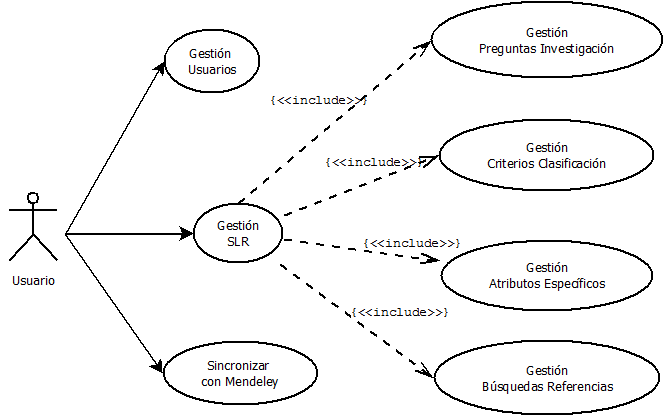
\includegraphics[scale=0.5]{cu-sistema.png}
		\caption{Diagrama casos de usos del sistema.}
		\label{fig:cu01}
	\end{center}
\end{figure}

\begin{figure}[hp!]
	\begin{center} 
		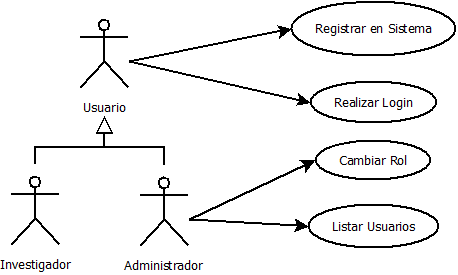
\includegraphics[scale=0.6]{cu-gestusuarios.png}
		\caption{Diagrama casos de usos de la gestión de usuarios.}
		\label{fig:cu02}
	\end{center}
\end{figure}

\begin{figure}[hp!]
	\begin{center}
		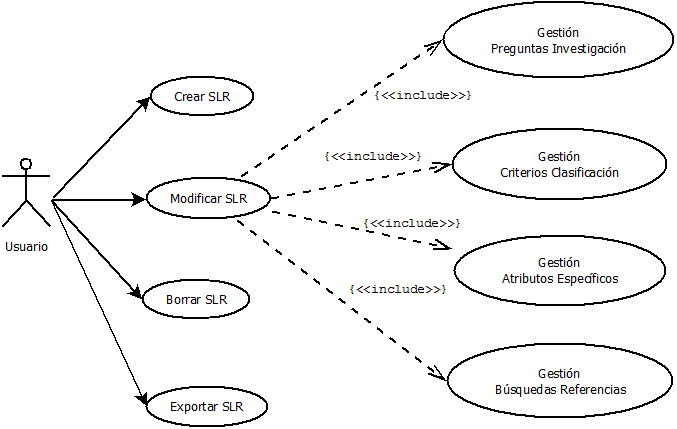
\includegraphics[scale=0.55]{cu-gestslr.png}
		\caption{Diagrama casos de usos de la gestión de revisiones sistemáticas.}
		\label{fig:cu03}
	\end{center}
\end{figure}

\begin{figure}[hp!]
	\begin{center}
		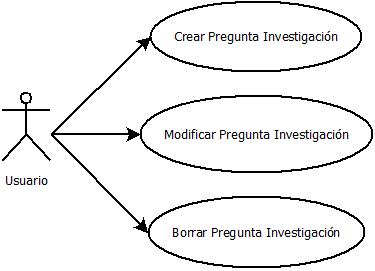
\includegraphics[scale=0.55]{cu-gestpreginv.png}
		\caption{Diagrama casos de usos de la gestión de preguntas de investigación.}
		\label{fig:cu04}
	\end{center}
\end{figure}

\begin{figure}[hp!]
	\begin{center}
		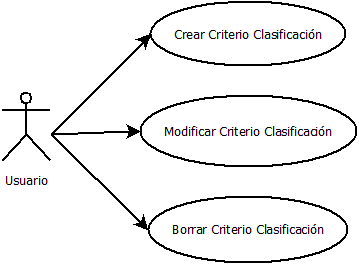
\includegraphics[scale=0.55]{cu-gestcrit.png}
		\caption{Diagrama casos de usos de la gestión de criterios de clasificación.}
		\label{fig:cu05}
	\end{center}
\end{figure}

\begin{figure}[hp!]
	\begin{center}
		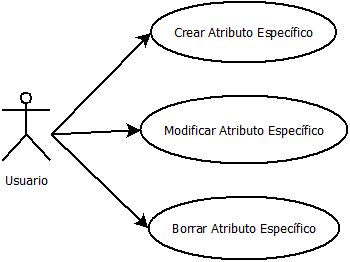
\includegraphics[scale=0.55]{cu-gestatesp.png}
		\caption{Diagrama casos de usos de la gestión de atributos específicos.}
		\label{fig:cu06}
	\end{center}
\end{figure}

\begin{figure}[hp!]
	\begin{center}
		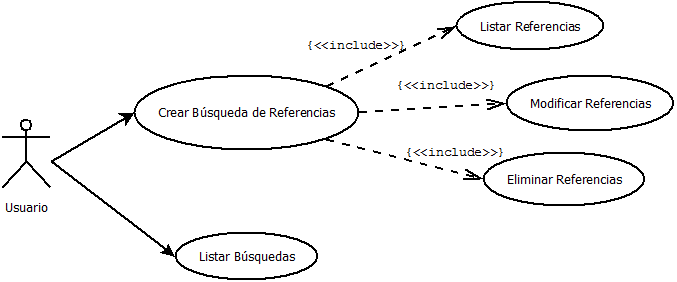
\includegraphics[scale=0.55]{cu-gestbusquedas.png}
		\caption{Diagrama casos de usos de la gestión de búsquedas de referencias bibliográficas.}
		\label{fig:cu07}
	\end{center}
\end{figure}

\newpage

\begin{figure}[hp!]
	\begin{center}
		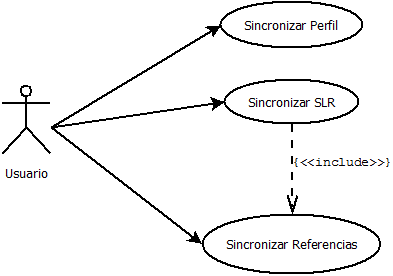
\includegraphics[scale=0.55]{cu-sincromend.png}
		\caption{Diagrama casos de usos de la sincronización con Mendeley.}
		\label{fig:cu08}
	\end{center}
\end{figure}

\begin{table}[!hbt]
	\begin{center}
		\begin{tabular}{|p{4cm}|p{11cm}|}
			\hline
			\textbf{Nombre} & CU-01 Registrar en sistema\\
			\hline
			\textbf{Descripción} & El usuario se registra en el sistema por primera vez para poder crear revisiones sistemáticas de la literatura.\\
			\hline
			\textbf{Precondición} & El usuario tiene una cuenta de Mendeley y no se ha logado antes en el sistema.\\
			\hline
			\textbf{Postcondición} & El usuario tiene acceso a la aplicación web.\\
			\hline
			\textbf{Actores} & Usuario\\
			\hline
			\textbf{Escenario principal} & 
				\begin{enumerate}
					\item El usuario introduce el email y contraseña de la cuenta Mendeley.
					\item El sistema valida que el email y la contraseña sean correctas redirigiendo al usuario a la pantalla principal de la aplicación web.
				\end{enumerate}
			\\
			\hline
			\textbf{\shortstack[l]{Escenarios \\ alternativos}} & 
				
				\begin{enumerate}[label=2 \alph*]
					%\setcounter{enumi}{2}
					\item El sistema verifica que el email y la contraseña no son correctas. Volvemos al paso 1.
				\end{enumerate}
			\\
			\hline
		\end{tabular}
		\caption{CU-01 Registar en sistema}
		\label{table:cu01}
	\end{center}
\end{table}

\begin{table}[!hbt]
	\begin{center}
		\begin{tabular}{|p{4cm}|p{11cm}|}
			\hline
			\textbf{Nombre} & CU-02 Realizar login\\
			\hline
			\textbf{Descripción} & El usuario se identifica en el sistema web.\\
			\hline
			\textbf{Precondición} & El usuario debe estar registrado en el sistema web.\\
			\hline
			\textbf{Postcondición} & El usuario tiene acceso a la aplicación web.\\
			\hline
			\textbf{Actores} & Usuario\\
			\hline
			\textbf{Escenario principal} & 
				\begin{enumerate}
					\item El usuario introduce el email y contraseña de la cuenta Mendeley.
					\item El sistema valida que el email y la contraseña sean correctas redirigiendo al usuario a la pantalla principal de la aplicación web.
				\end{enumerate}
			\\
			\hline
			\textbf{\shortstack[l]{Escenarios \\ alternativos}} & 
				
				\begin{enumerate}[label=2 \alph*]
					%\setcounter{enumi}{2}
					\item El sistema verifica que el email y la contraseña no son correctas. Volvemos al paso 1.
				\end{enumerate}
			\\
			\hline
		\end{tabular}
		\caption{CU-02 Realizar login}
		\label{table:cu02}
	\end{center}
\end{table}

\begin{table}[!hbt]
	\begin{center}
		\begin{tabular}{|p{4cm}|p{11cm}|}
			\hline
			\textbf{Nombre} & CU-03 Cambiar rol\\
			\hline
			\textbf{Descripción} & El administrador del sistema puede cambiar de rol a otro usuario.\\
			\hline
			\textbf{Precondición} & El usuario debe estar logado en el sistema y poseer rol administrador.\\
			\hline
			\textbf{Postcondición} & El administrador cambiar de rol a otro usuario.\\
			\hline
			\textbf{Actores} & Administrador\\
			\hline
			\textbf{Escenario principal} & 
				\begin{enumerate}
					\item El administrador del sistema busca al usuario a través de su email.
					\item El sistema ofrece toda la información del usuario.
					\item El administrador selecciona la opción de cambiar de rol al usuario.
					\item El sistema realiza el cambio y muestra un mensaje de que el proceso se ha realizado correctamente.
				\end{enumerate}
			\\
			\hline
			\textbf{\shortstack[l]{Escenarios \\ alternativos}} & --
			\\
			\hline
		\end{tabular}
		\caption{CU-03 Cambiar rol}
		\label{table:cu03}
	\end{center}
\end{table}

\begin{table}[!hbt]
	\begin{center}
		\begin{tabular}{|p{4cm}|p{11cm}|}
			\hline
			\textbf{Nombre} & CU-04 Listar Usuarios\\
			\hline
			\textbf{Descripción} & El administrador puede obtener una lista de todos los usuarios registrados en la aplicación web.\\
			\hline
			\textbf{Precondición} & El administrador está logado en el sistema y tiene rol administrador.\\
			\hline
			\textbf{Postcondición} & El administrador obtiene un listado completo de los usuarios registrados en el sistema.\\
			\hline
			\textbf{Actores} & Administrador\\
			\hline
			\textbf{Escenario principal} & 
				\begin{enumerate}
					\item El administrador elige la opción de listado de usuarios.
					\item El sistema muestra el listado de todos los usuarios registrados en la aplicación.
				\end{enumerate}
			\\
			\hline
			\textbf{\shortstack[l]{Escenarios \\ alternativos}} & --\\
			\hline
		\end{tabular}
		\caption{CU-04 Listar usuarios}
		\label{table:cu04}
	\end{center}
\end{table}

\begin{table}[!hbt]
	\begin{center}
		\begin{tabular}{|p{4cm}|p{11cm}|}
			\hline
			\textbf{Nombre} & CU-05 Crear SLR\\
			\hline
			\textbf{Descripción} & El usuario elige la opción de crear una revisión sistemática de la literatura.\\
			\hline
			\textbf{Precondición} & El usuario debe estar registrado en el sistema web.\\
			\hline
			\textbf{Postcondición} & El usuario crea una revisión sistemática de la literatura.\\
			\hline
			\textbf{Actores} & Usuario\\
			\hline
			\textbf{Escenario principal} & 
				\begin{enumerate}
					\item El usuario elige la opción Crear SLR.
					\item El sistema muestra una ventana donde se debe insertar el título y la justificación del mismo.
					\item El usuario introduce el título y justificación del SLR a crear.
					\item El sistema comprueba que no haya un SLR con el mismo título y que el formato del mismo sea correcto mostrando un mensaje de confirmación de la creación del SLR.
				\end{enumerate}
			\\
			\hline
			\textbf{\shortstack[l]{Escenarios \\ alternativos}} & 
				
				\begin{enumerate}[label=4 \alph*]
					%\setcounter{enumi}{2}
					\item El sistema verifica que el título no cumple el formato correcto o el título está siendo usado por otro SLR. Volvemos al paso 2.
				\end{enumerate}
			\\
			\hline
		\end{tabular}
		\caption{CU-05 Crear SLR}
		\label{table:cu05}
	\end{center}
\end{table}

\begin{table}[!hbt]
	\begin{center}
		\begin{tabular}{|p{4cm}|p{11cm}|}
			\hline
			\textbf{Nombre} & CU-06 Modificar SLR\\
			\hline
			\textbf{Descripción} & El usuario puede realizar modificaciones de una revisión sistemática de la literatura realizando operaciones sobre las preguntas de investigación, criterios de clasificación, atributos específicos o búsquedas de referencias.\\
			\hline
			\textbf{Precondición} & El usuario debe estar registrado en el sistema web y el SLR a modificar existe.\\
			\hline
			\textbf{Postcondición} & El usuario modifica una revisión sistemática de la literatura.\\
			\hline
			\textbf{Actores} & Usuario\\
			\hline
			\textbf{Escenario principal} & 
				\begin{enumerate}
					\item El usuario realiza operaciones sobre las preguntas de investigación: \ref{table:cu09}, \ref{table:cu10}, \ref{table:cu11}.
					\item El usuario realiza operaciones sobre los criterios de clasificación: \ref{table:cu12}, \ref{table:cu13}, \ref{table:cu14}, .
					\item El usuario realiza operaciones sobre los atributos específicos: \ref{table:cu15}, \ref{table:cu16}, \ref{table:cu17}.
					\item El usuario realiza operaciones sobre las búsquedas de referencias \ref{table:cu18}
				\end{enumerate}
			\\
			\hline
			\textbf{\shortstack[l]{Escenarios \\ alternativos}} & Ver escenarios alternativos de casos de uso..\\
			\hline
		\end{tabular}
		\caption{CU-06 Modificar SLR}
		\label{table:cu06}
	\end{center}
\end{table}

\begin{table}[!hbt]
	\begin{center}
		\begin{tabular}{|p{4cm}|p{11cm}|}
			\hline
			\textbf{Nombre} & CU-07 Borrar SLR\\
			\hline
			\textbf{Descripción} & El usuario elige la opción de borrar una revisión sistemática de la literatura.\\
			\hline
			\textbf{Precondición} & El usuario debe estar registrado en el sistema web y el SLR a borrar existe.\\
			\hline
			\textbf{Postcondición} & El usuario borra una revisión sistemática de la literatura del sistema.\\
			\hline
			\textbf{Actores} & Usuario\\
			\hline
			\textbf{Escenario principal} & 
				\begin{enumerate}
					\item El usuario elige la opción Borrar SLR.
					\item El sistema muestra una ventana donde pregunta al cliente si confirma el borrado de la revisión sistemática de la literatura.
					\item El usuario confirma el borrado del SLR.
					\item El sistema elimina el SLR del sistema mostrando un mensaje de confirmación del borrado.
				\end{enumerate}
			\\
			\hline
			\textbf{\shortstack[l]{Escenarios \\ alternativos}} & 
				
				\begin{enumerate}[label=3 \alph*]
					%\setcounter{enumi}{2}
					\item El usuario elige la opción Cancelar. El sistema mostrará un listado de las revisiones sistemáticas del usuario.
				\end{enumerate}
			\\
			\hline
		\end{tabular}
		\caption{CU-07 Borrar SLR}
		\label{table:cu07}
	\end{center}
\end{table}

\begin{table}[!hbt]
	\begin{center}
		\begin{tabular}{|p{4cm}|p{11cm}|}
			\hline
			\textbf{Nombre} & CU-08 Exportar SLR\\
			\hline
			\textbf{Descripción} & El usuario elige la opción de exportar datos de una revisión sistemática de la literatura.\\
			\hline
			\textbf{Precondición} & El usuario debe estar registrado en el sistema web y la revisión sistemática de la literatura debe ser propia del mismo.\\
			\hline
			\textbf{Postcondición} & El usuario obtiene los datos de una revisión sistemática de la literatura a través de un fichero de salida.\\
			\hline
			\textbf{Actores} & Usuario\\
			\hline
			\textbf{Escenario principal} & 
				\begin{enumerate}
					\item El usuario elige la opción de exportar una revisión sistemática de la literatura a través de un fichero o a través de gráficos.
					\item El sistema exporta los datos en el formato elegido por el usuario.
				\end{enumerate}
			\\
			\hline
			\textbf{\shortstack[l]{Escenarios \\ alternativos}} & --\\
			\hline
		\end{tabular}
		\caption{CU-08 Exportar SLR}
		\label{table:cu08}
	\end{center}
\end{table}

\begin{table}[!hbt]
	\begin{center}
		\begin{tabular}{|p{4cm}|p{11cm}|}
			\hline
			\textbf{Nombre} & CU-09 Crear Pregunta de investigación\\
			\hline
			\textbf{Descripción} & El usuario puede introducir preguntas de investigación en una revisión sistemática de la literatura.\\
			\hline
			\textbf{Precondición} & El usuario debe estar registrado en el sistema web y la revisión sistemática debe ser propia del usuario.\\
			\hline
			\textbf{Postcondición} & El usuario introduce una pregunta de investigación en una revisión sistemática de la literatura.\\
			\hline
			\textbf{Actores} & Usuario\\
			\hline
			\textbf{Escenario principal} & 
				\begin{enumerate}
					\item El usuario elige la opción Insertar Pregunta de Investigación.
					\item El sistema pide por pantalla el enunciado de la pregunta.
					\item El usuario introduce el enunciado de la pregunta.
					\item El sistema comprueba que el enunciado cumpla un formato y muestra un mensaje satisfactorio de la creación.
				\end{enumerate}
			\\
			\hline
			\textbf{\shortstack[l]{Escenarios \\ alternativos}} & 
				
				\begin{enumerate}[label=4 \alph*]
					%\setcounter{enumi}{2}
					\item El sistema verifica que el enunciado no cumple el formato. El sistema muestra un mensaje de error y se vuelve al paso 2.
				\end{enumerate}
			\\
			\hline
		\end{tabular}
		\caption{CU-09 Crear Pregunta de investigación}
		\label{table:cu09}
	\end{center}
\end{table}

\begin{table}[!hbt]
	\begin{center}
		\begin{tabular}{|p{4cm}|p{11cm}|}
			\hline
			\textbf{Nombre} & CU-10 Modificar Pregunta de investigación\\
			\hline
			\textbf{Descripción} & El usuario elige la opción de modificar una pregunta de investigación de una revisión sistemática de la literatura elegida.\\
			\hline
			\textbf{Precondición} & El usuario debe estar registrado en el sistema web y ser proprietario de la revisión sistemática de la literatura.\\
			\hline
			\textbf{Postcondición} & El usuario modifica la pregunta de investigación de un determinado SLR.\\
			\hline
			\textbf{Actores} & Usuario\\
			\hline
			\textbf{Escenario principal} & 
				\begin{enumerate}
					\item El usuario elige la opción modificar pregunta de investigación.
					\item El sistema muestra una pantalla con el enunciado de la pregunta a modificar.
					\item El usuario introduce el enunciado de la pregunta a modificar.
					\item El sistema comprueba que el enunciado de la pregunta cumple un formato y muestra un mensaje de confirmación al usuario.
				\end{enumerate}
			\\
			\hline
			\textbf{\shortstack[l]{Escenarios \\ alternativos}} & 
				
				\begin{enumerate}[label=4 \alph*]
					%\setcounter{enumi}{2}
					\item El sistema verifica que el enunciado no cumple un formato correcto. Volvemos al paso 2 junto con un mensaje de alerta al usuario.
				\end{enumerate}
			\\
			\hline
		\end{tabular}
		\caption{CU-10 Modificar pregunta de investigación}
		\label{table:cu10}
	\end{center}
\end{table}

\begin{table}[!hbt]
	\begin{center}
		\begin{tabular}{|p{4cm}|p{11cm}|}
			\hline
			\textbf{Nombre} & CU-11 Borrar pregunta de investigación\\
			\hline
			\textbf{Descripción} & El usuario elige la opción de borrar una pregunta de investigación de una revisión sistemática.\\
			\hline
			\textbf{Precondición} & El usuario debe estar registrado en el sistema web y ser proprietario de la revisión sistemática.\\
			\hline
			\textbf{Postcondición} & El usuario realiza el borrado de una pregunta de investigación.\\
			\hline
			\textbf{Actores} & Usuario\\
			\hline
			\textbf{Escenario principal} & 
				\begin{enumerate}
					\item El usuario elige la opción Borrar pregunta de investigación.
					\item El sistema muestra una ventana donde se pide la confirmación de la pregunta de investigación.
					\item El usuario realiza la confirmación del borrado.
					\item El sistema borra la pregunta del sistema y muestra un mensaje de confirmación del borrado al usuario.
				\end{enumerate}
			\\
			\hline
			\textbf{\shortstack[l]{Escenarios \\ alternativos}} & -- \\
			\hline
		\end{tabular}
		\caption{CU-11 Borrar pregunta investigación}
		\label{table:cu11}
	\end{center}
\end{table}

\begin{table}[!hbt]
	\begin{center}
		\begin{tabular}{|p{4cm}|p{11cm}|}
			\hline
			\textbf{Nombre} & CU-12 Crear Criterio de clasificación\\
			\hline
			\textbf{Descripción} & El usuario elige la opción de crear un criterio de clasificación de referencias.\\
			\hline
			\textbf{Precondición} & El usuario debe estar registrado en el sistema web y ser proprietario de la revisión sistemática de la literatura.\\
			\hline
			\textbf{Postcondición} & El usuario crea un criterio de clasificación de referencias.\\
			\hline
			\textbf{Actores} & Usuario\\
			\hline
			\textbf{Escenario principal} & 
				El escenario principal es el mismo que el \ref{table:cu09} pero adaptado a los criterios de clasificación de referencias.
			\\
			\hline
			\textbf{\shortstack[l]{Escenarios \\ alternativos}} & 
				
				Los escenarios alternativos son los mismos que el \ref{table:cu09} pero adaptados a los criterios de clasificación de referencias.
			\\
			\hline
		\end{tabular}
		\caption{CU-12 Crear criterio de clasificación}
		\label{table:cu12}
	\end{center}
\end{table}

\begin{table}[!hbt]
	\begin{center}
		\begin{tabular}{|p{4cm}|p{11cm}|}
			\hline
			\textbf{Nombre} & CU-13 Modificar Criterio de clasificación\\
			\hline
			\textbf{Descripción} & El usuario elige la opción de modificar un criterio de clasificación de referencias.\\
			\hline
			\textbf{Precondición} & El usuario debe estar registrado en el sistema web y ser proprietario de la revisión sistemática de la literatura.\\
			\hline
			\textbf{Postcondición} & El usuario modifica un criterio de clasificación de referencias.\\
			\hline
			\textbf{Actores} & Usuario\\
			\hline
			\textbf{Escenario principal} & 
				El escenario principal es el mismo que el \ref{table:cu10} pero adaptado a los criterios de clasificación de referencias.
			\\
			\hline
			\textbf{\shortstack[l]{Escenarios \\ alternativos}} & 
				
				Los escenarios alternativos son los mismos que el \ref{table:cu10} pero adaptados a los criterios de clasificación de referencias.
			\\
			\hline
		\end{tabular}
		\caption{CU-13 Modificar criterio de clasificación}
		\label{table:cu13}
	\end{center}
\end{table}

\begin{table}[!hbt]
	\begin{center}
		\begin{tabular}{|p{4cm}|p{11cm}|}
			\hline
			\textbf{Nombre} & CU-14 Borrar Criterio de clasificación\\
			\hline
			\textbf{Descripción} & El usuario elige la opción de borrar un criterio de clasificación de referencias.\\
			\hline
			\textbf{Precondición} & El usuario debe estar registrado en el sistema web y ser proprietario de la revisión sistemática de la literatura.\\
			\hline
			\textbf{Postcondición} & El usuario borra un criterio de clasificación de referencias.\\
			\hline
			\textbf{Actores} & Usuario\\
			\hline
			\textbf{Escenario principal} & 
			
			\begin{itemize}
				\item El escenario principal es el mismo que el \ref{table:cu11} pero adaptado a los criterios de clasificación de referencias.
				\item Todas las referencias bibliográficas que contengan dicha referencia, tendrán un nuevo criterio 'incluido'.
			\end{itemize}
			\\
			\hline
			\textbf{\shortstack[l]{Escenarios \\ alternativos}} & 
				
				Los escenarios alternativos son los mismos que el \ref{table:cu11} pero adaptados a los criterios de clasificación de referencias.
			\\
			\hline
		\end{tabular}
		\caption{CU-14 Borrar criterio de clasificación}
		\label{table:cu14}
	\end{center}
\end{table}

\begin{table}[!hbt]
	\begin{center}
		\begin{tabular}{|p{4cm}|p{11cm}|}
			\hline
			\textbf{Nombre} & CU-15 Crear atributo específico\\
			\hline
			\textbf{Descripción} & El usuario elige la opción de crear un atributo específico.\\
			\hline
			\textbf{Precondición} & El usuario debe estar registrado en el sistema web y ser proprietario de la revisión sistemática de la literatura.\\
			\hline
			\textbf{Postcondición} & El usuario crea un atributo específico para las referencias de un slr.\\
			\hline
			\textbf{Actores} & Usuario\\
			\hline
			\textbf{Escenario principal} & 
				El escenario principal es el mismo que el \ref{table:cu09} pero adaptado a los atributos específicos.
			\\
			\hline
			\textbf{\shortstack[l]{Escenarios \\ alternativos}} & 
				
				Los escenarios alternativos son los mismos que el \ref{table:cu09} pero adaptados a los atributos específicos.
			\\
			\hline
		\end{tabular}
		\caption{CU-15 Crear atributo específico}
		\label{table:cu15}
	\end{center}
\end{table}

\begin{table}[!hbt]
	\begin{center}
		\begin{tabular}{|p{4cm}|p{11cm}|}
			\hline
			\textbf{Nombre} & CU-16 Modificar atributo específico\\
			\hline
			\textbf{Descripción} & El usuario elige la opción de modificar atributo específico.\\
			\hline
			\textbf{Precondición} & El usuario debe estar registrado en el sistema web y ser proprietario de la revisión sistemática de la literatura.\\
			\hline
			\textbf{Postcondición} & El usuario modifica un atributo específico.\\
			\hline
			\textbf{Actores} & Usuario\\
			\hline
			\textbf{Escenario principal} & 
				El escenario principal es el mismo que el \ref{table:cu10} pero adaptado a los atributos específicos.
			\\
			\hline
			\textbf{\shortstack[l]{Escenarios \\ alternativos}} & 
				
				Los escenarios alternativos son los mismos que el \ref{table:cu09} pero adaptados a los criterios de clasificación de referencias.
			\\
			\hline
		\end{tabular}
		\caption{CU-16 Modificar atributo de especificación}
		\label{table:cu16}
	\end{center}
\end{table}

\begin{table}[!hbt]
	\begin{center}
		\begin{tabular}{|p{4cm}|p{11cm}|}
			\hline
			\textbf{Nombre} & CU-17 Borrar atributo específico\\
			\hline
			\textbf{Descripción} & El usuario elige la opción de eliminar atributo específico.\\
			\hline
			\textbf{Precondición} & El usuario debe estar registrado en el sistema web y ser proprietario de la revisión sistemática de la literatura.\\
			\hline
			\textbf{Postcondición} & El usuario elimina un atributo específico.\\
			\hline
			\textbf{Actores} & Usuario\\
			\hline
			\textbf{Escenario principal} & 
				El escenario principal es el mismo que el \ref{table:cu11} pero adaptado a los atributos específicos.
			\\
			\hline
			\textbf{\shortstack[l]{Escenarios \\ alternativos}} & 
				
				Los escenarios alternativos son los mismos que el \ref{table:cu11} pero adaptados a los criterios de clasificación de referencias.
			\\
			\hline
		\end{tabular}
		\caption{CU-17 Eliminar atributo de especificación}
		\label{table:cu17}
	\end{center}
\end{table}

\begin{table}[!hbt]
	\begin{center}
		\begin{tabular}{|p{4cm}|p{11cm}|}
			\hline
			\textbf{Nombre} & CU-18 Crear búsquedas de referencias\\
			\hline
			\textbf{Descripción} & El usuario elige la opción de crear una búsqueda de referencias.\\
			\hline
			\textbf{Precondición} & El usuario debe estar registrado en el sistema web y ser proprietario de la revisión sistemática de la literatura.\\
			\hline
			\textbf{Postcondición} & El usuario realiza una búsqueda de referencias.\\
			\hline
			\textbf{Actores} & Usuario\\
			\hline
			\textbf{Escenario principal} & 
				
				\begin{enumerate}
					\item El usuario elige la opción de creación de una búsqueda de referencias
					\item El sistema muestra todos los campos que debe de rellenar.
					\item El usuario introduce los términos de búsquedas, elige los motores de búsquedas, el total de referencias a buscar y en qué intervalo de años deben pertenecer.
					\item El sistema realiza la búsqueda, indicando el estado de la misma y confirmando que se ha realizado correctamente cuando la búsqueda ha sido finalizada.
				\end{enumerate}
			\\
			\hline
			\textbf{\shortstack[l]{Escenarios \\ alternativos}} & 
				
				\begin{enumerate}[label=4 \alph*]
					%\setcounter{enumi}{2}
					\item El sistema ha detectado algún error en el formato de los datos de entrada. El sistema alerta al usuario y se vuelve al paso 3.
					\item El sistema no puede realizar una búsqueda debido a problemas de conexión con los motores de búsquedas. El sistema guarda el error, advierte al usuario y el administrador del sistema puede gestionarlo.
				\end{enumerate}
			\\
			\hline
		\end{tabular}
		\caption{CU-18 Crear búsquedas de referencias}
		\label{table:cu18}
	\end{center}
\end{table}

\begin{table}[!hbt]
	\begin{center}
		\begin{tabular}{|p{4cm}|p{11cm}|}
			\hline
			\textbf{Nombre} & CU-19 Listar Referencias\\
			\hline
			\textbf{Descripción} & El usuario elige la opción de listar las referencias bibliográficas.\\
			\hline
			\textbf{Precondición} & El usuario debe estar registrado en el sistema web y ser proprietario de la revisión sistemática de la literatura.\\
			\hline
			\textbf{Postcondición} & El usuario lista todas las referencias bibliográficas de una revisión sistemática de la literatura.\\
			\hline
			\textbf{Actores} & Usuario\\
			\hline
			\textbf{Escenario principal} & 
				
				\begin{enumerate}
					\item El usuario elige la opción de listar las referencias.
					\item El sistema muestra todas las referencias bibliográficas que pertenecen a una revisión sistemática.
				\end{enumerate}
			\\
			\hline
			\textbf{\shortstack[l]{Escenarios \\ alternativos}} &  --\\
			\hline
		\end{tabular}
		\caption{CU-19 Listar referencias}
		\label{table:cu19}
	\end{center}
\end{table}

\begin{table}[!hbt]
	\begin{center}
		\begin{tabular}{|p{4cm}|p{11cm}|}
			\hline
			\textbf{Nombre} & CU-20 Modificar referencias\\
			\hline
			\textbf{Descripción} & El usuario elige la opción de modificar referencias bibliográficas.\\
			\hline
			\textbf{Precondición} & El usuario debe estar registrado en el sistema web y ser proprietario de la revisión sistemática de la literatura.\\
			\hline
			\textbf{Postcondición} & El usuario modifica una referencia bibliográfica.\\
			\hline
			\textbf{Actores} & Usuario\\
			\hline
			\textbf{Escenario principal} & 
				El escenario principal es el mismo que el \ref{table:cu10} pero adaptado a las referencias bibliográficas.
			\\
			\hline
			\textbf{\shortstack[l]{Escenarios \\ alternativos}} & 
				
				Los escenarios alternativos son los mismos que el \ref{table:cu10} pero adaptados a las referencias bibliográficas.
			\\
			\hline
		\end{tabular}
		\caption{CU-20 Modificar referencias}
		\label{table:cu20}
	\end{center}
\end{table}

\begin{table}[!hbt]
	\begin{center}
		\begin{tabular}{|p{4cm}|p{11cm}|}
			\hline
			\textbf{Nombre} & CU-21 Eliminar referencias\\
			\hline
			\textbf{Descripción} & El usuario elige la opción de eliminar referencias bibliográficas.\\
			\hline
			\textbf{Precondición} & El usuario debe estar registrado en el sistema web y ser proprietario de la revisión sistemática de la literatura.\\
			\hline
			\textbf{Postcondición} & El usuario elimina una referencia bibliográfica.\\
			\hline
			\textbf{Actores} & Usuario\\
			\hline
			\textbf{Escenario principal} & 
				El escenario principal es el mismo que el \ref{table:cu11} pero adaptado a las referencias bibliográficas.
			\\
			\hline
			\textbf{\shortstack[l]{Escenarios \\ alternativos}} & 
				
				Los escenarios alternativos son los mismos que el \ref{table:cu11} pero adaptados a las referencias bibliográficas.
			\\
			\hline
		\end{tabular}
		\caption{CU-21 Eliminar referencias}
		\label{table:cu21}
	\end{center}
\end{table}

\begin{table}[!hbt]
	\begin{center}
		\begin{tabular}{|p{4cm}|p{11cm}|}
			\hline
			\textbf{Nombre} & CU-22 Listar Búsquedas\\
			\hline
			\textbf{Descripción} & El usuario elige la opción de listar las búsquedas realizadas en una revisión sistemática de la literatura.\\
			\hline
			\textbf{Precondición} & El usuario debe estar registrado en el sistema web y ser proprietario de la revisión sistemática de la literatura.\\
			\hline
			\textbf{Postcondición} & El usuario lista todas las búsquedas de una revisión sistemática de la literatura.\\
			\hline
			\textbf{Actores} & Usuario\\
			\hline
			\textbf{Escenario principal} & 
				
				El escenario principal es el mismo que el de \ref{table:cu19} pero adaptado a las búsquedas de una revisión sistemática de la literatura.
			\\
			\hline
			\textbf{\shortstack[l]{Escenarios \\ alternativos}} &  Los escenarios alternativos son los mismos que los de \ref{table:cu19} pero adaptados a las búsquedas de una revisión sistemática de la literatura.\\
			\hline
		\end{tabular}
		\caption{CU-22 Listar Búsquedas}
		\label{table:cu22}
	\end{center}
\end{table}

\begin{table}[!hbt]
	\begin{center}
		\begin{tabular}{|p{4cm}|p{11cm}|}
			\hline
			\textbf{Nombre} & CU-23 Sincronizar perfil\\
			\hline
			\textbf{Descripción} & El usuario elige la opción de sincronizar los datos de su perfil con los que tiene almacenados en su cuenta de Mendeley.\\
			\hline
			\textbf{Precondición} & El usuario debe estar registrado en el sistema web.\\
			\hline
			\textbf{Postcondición} & El usuario sincroniza los datos de su perfil.\\
			\hline
			\textbf{Actores} & Usuario\\
			\hline
			\textbf{Escenario principal} & 
				\begin{enumerate}
					\item El usuario elige la opción Sincronizar Perfil.
					\item El sistema conecta vía API REST con Mendeley y actualiza la información con los datos que proporciona Mendeley. El sistema además, mostrará un mensaje de confirmación.
				\end{enumerate}
			\\
			\hline
			\textbf{\shortstack[l]{Escenarios \\ alternativos}} & 
			
				\begin{enumerate}[label=2 \alph*]
						%\setcounter{enumi}{2}
						\item El sistema detecta un error de sincronización. El sistema avisa al usuario y le indica que debe intentarlo más tarde.
					\end{enumerate}
					
			\\
			\hline
		\end{tabular}
		\caption{CU-23 Sincronizar Perfil}
		\label{table:cu23}
	\end{center}
\end{table}

\begin{table}[!hbt]
	\begin{center}
		\begin{tabular}{|p{4cm}|p{11cm}|}
			\hline
			\textbf{Nombre} & CU-24 Sincronizar SLR\\
			\hline
			\textbf{Descripción} & El usuario elige la opción de sincronizar los datos de un SLR con los proporcionados por Mendeley.\\
			\hline
			\textbf{Precondición} & El usuario debe estar registrado en el sistema web y ser proprietario de la revisión sistemática de la literatura.\\
			\hline
			\textbf{Postcondición} & El usuario sincroniza los datos del SLR.\\
			\hline
			\textbf{Actores} & Usuario\\
			\hline
			\textbf{Escenario principal} & 
				El escenario principal es el mismo que \ref{table:cu23} pero adaptado a las revisiones sistemáticas de la literatura.
			\\
			\hline
			\textbf{\shortstack[l]{Escenarios \\ alternativos}} & 
			
				Los escenarios alternativos son los mismos que \ref{table:cu23} pero adaptados a las revisiones sistemáticas de la literatura.
					
			\\
			\hline
		\end{tabular}
		\caption{CU-24 Sincronizar SLR}
		\label{table:cu24}
	\end{center}
\end{table}

\begin{table}[!hbt]
	\begin{center}
		\begin{tabular}{|p{4cm}|p{11cm}|}
			\hline
			\textbf{Nombre} & CU-25 Sincronizar Referencias\\
			\hline
			\textbf{Descripción} & El usuario elige la opción de sincronizar los datos de una referencia con los proporcionados por Mendeley.\\
			\hline
			\textbf{Precondición} & El usuario debe estar registrado en el sistema web y ser proprietario de la revisión sistemática de la literatura.\\
			\hline
			\textbf{Postcondición} & El usuario sincroniza los datos de la referencia\\
			\hline
			\textbf{Actores} & Usuario\\
			\hline
			\textbf{Escenario principal} & 
				El escenario principal es el mismo que \ref{table:cu23} pero adaptado a las referencias bibliográficas.
			\\
			\hline
			\textbf{\shortstack[l]{Escenarios \\ alternativos}} & 
			
				Los escenarios alternativos son los mismos que \ref{table:cu23} pero adaptados a las referencias bibliográficas.
					
			\\
			\hline
		\end{tabular}
		\caption{CU-24 Sincronizar Referencias}
		\label{table:cu25}
	\end{center}
\end{table}

%\section{Modelo de Comportamiento}
%A partir de los casos de uso anteriores, se crea el modelo de comportamiento. Para ello, se realizarán los diagramas de secuencia del sistema, donde se identificarán las operaciones o servicios del sistema. Luego, se detallará el contrato de las operaciones identificadas.

\clearpage
\newpage

\section{Modelo de Interfaz de Usuario}
En esta sección se incluye un prototipo de baja fidelidad (\textit{mockup}) de la interfaz de usuario del sistema. Se han realizado \textit{mockups} medio de \textit{Balsamiq} \cite{mybalsamiq}. En las figuras \ref{fig:mock01}, \ref{fig:mock02}, \ref{fig:mock03}, \ref{fig:mock04}, \ref{fig:mock05}, \ref{fig:mock06}, \ref{fig:mock07}, \ref{fig:mock08} y \ref{fig:mock09} podemos ver algunas de estas interfaces del usuario.\\

\begin{figure}[!hp]
	\begin{center} 
		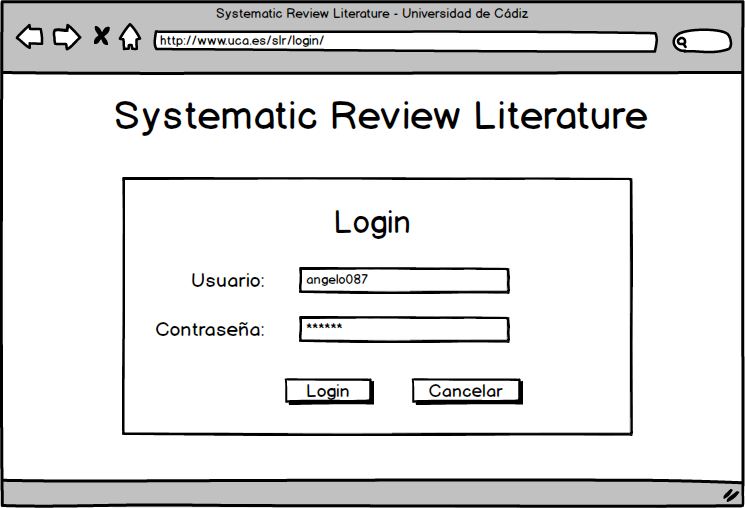
\includegraphics[scale=0.3]{mock01.png}
		\caption{Pantalla login.}
		\label{fig:mock01}
	\end{center}
\end{figure}

\begin{figure}[!hp]
	\begin{center} 
		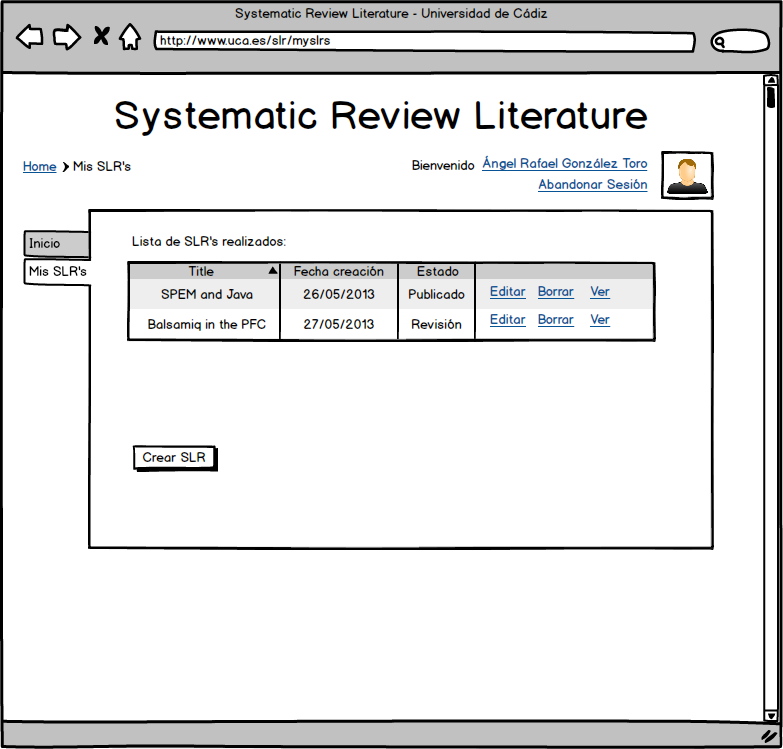
\includegraphics[scale=0.3]{mock02.png}
		\caption{Pantalla Revisiones Sistemáticas Usuario.}
		\label{fig:mock02}
	\end{center}
\end{figure}

\begin{figure}[!hp]
	\begin{center} 
		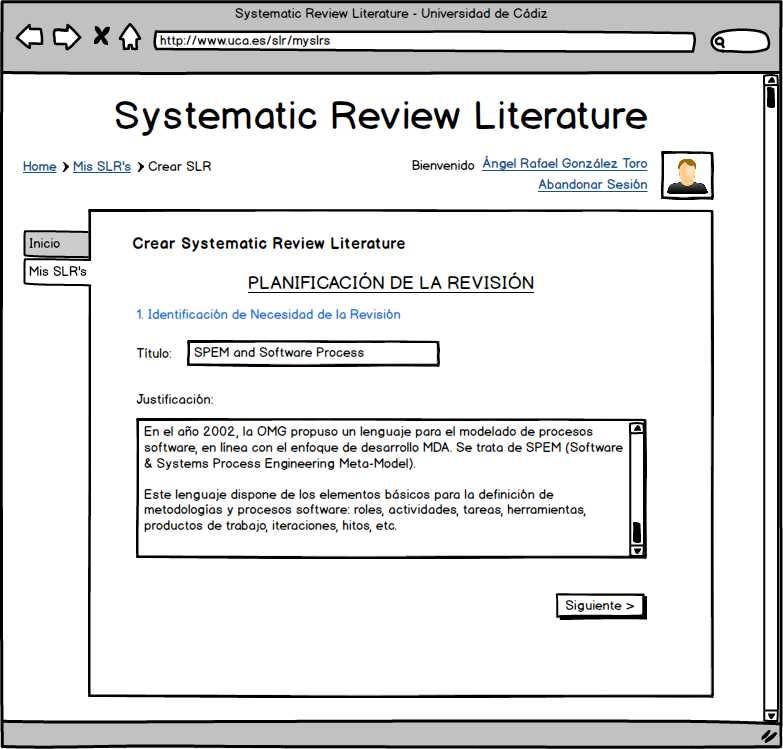
\includegraphics[scale=0.3]{mock03.png}
		\caption{Pantalla creación revisión sistemática}
		\label{fig:mock03}
	\end{center}
\end{figure}

\begin{figure}[!hp]
	\begin{center} 
		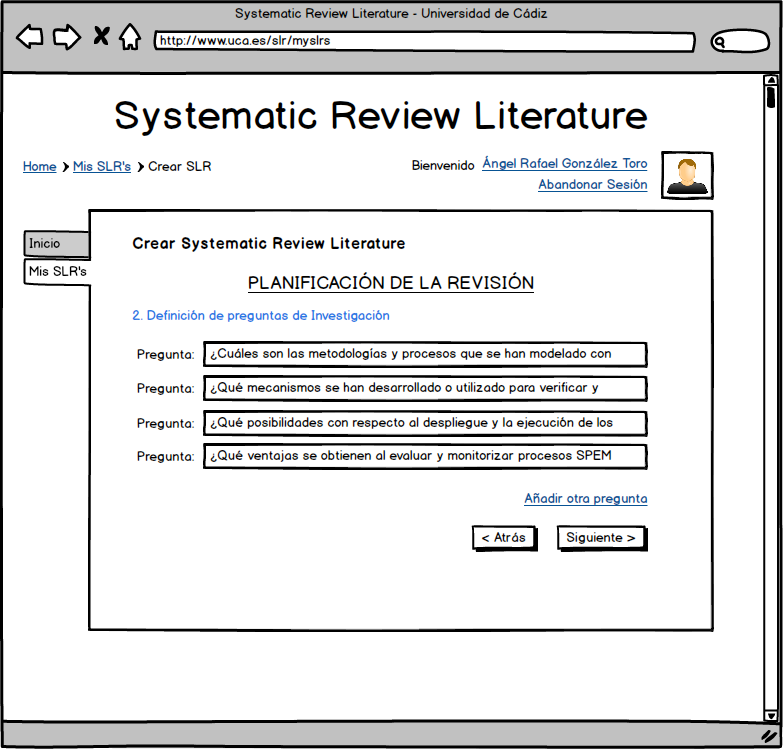
\includegraphics[scale=0.3]{mock04.png}
		\caption{Pantalla creación preguntas de investigación}
		\label{fig:mock04}
	\end{center}
\end{figure}

\begin{figure}[!hp]
	\begin{center} 
		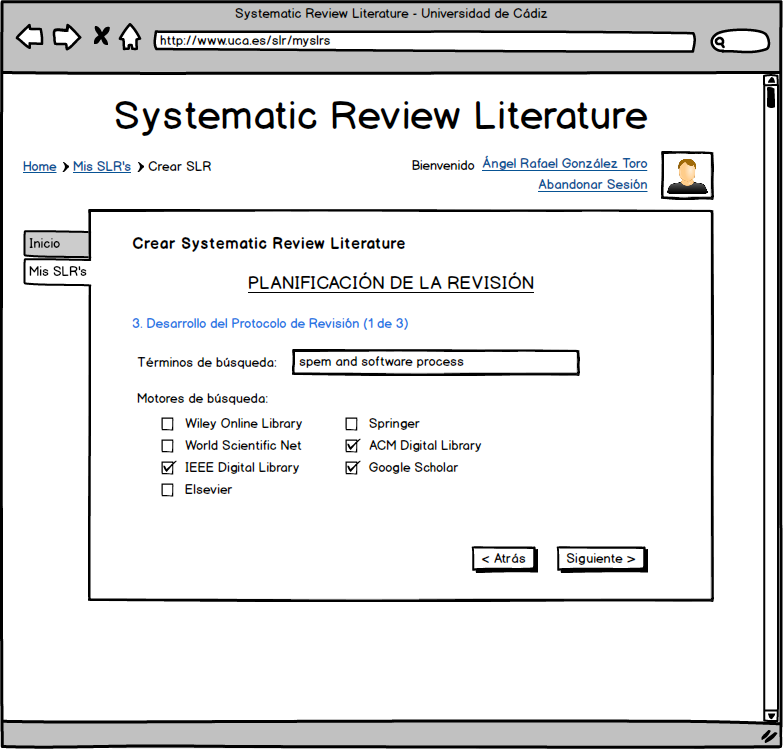
\includegraphics[scale=0.3]{mock05.png}
		\caption{Pantalla creación búsquedas de referencias bibliográficas.}
		\label{fig:mock05}
	\end{center}
\end{figure}

\begin{figure}[!hp]
	\begin{center} 
		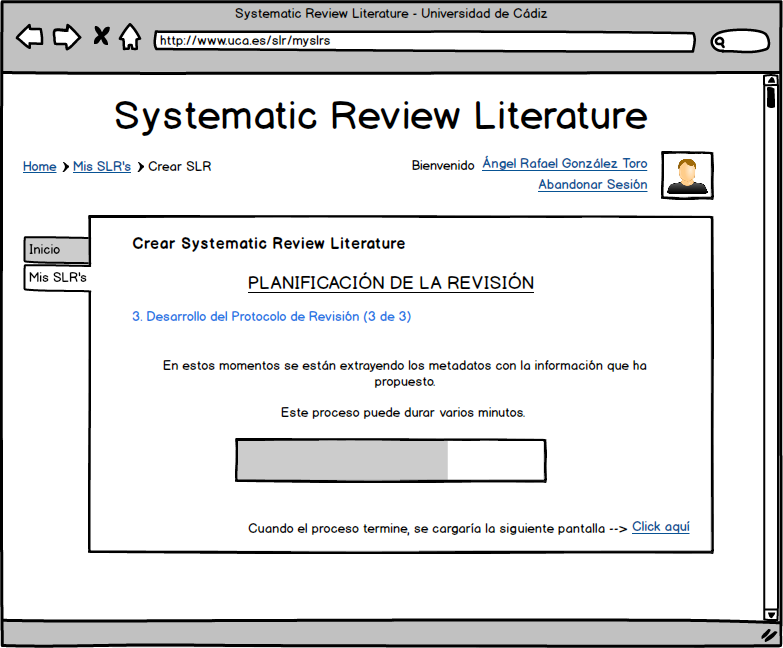
\includegraphics[scale=0.3]{mock06.png}
		\caption{Pantalla de creación de búsquedas en progreso.}
		\label{fig:mock06}
	\end{center}
\end{figure}

\begin{figure}[!hp]
	\begin{center} 
		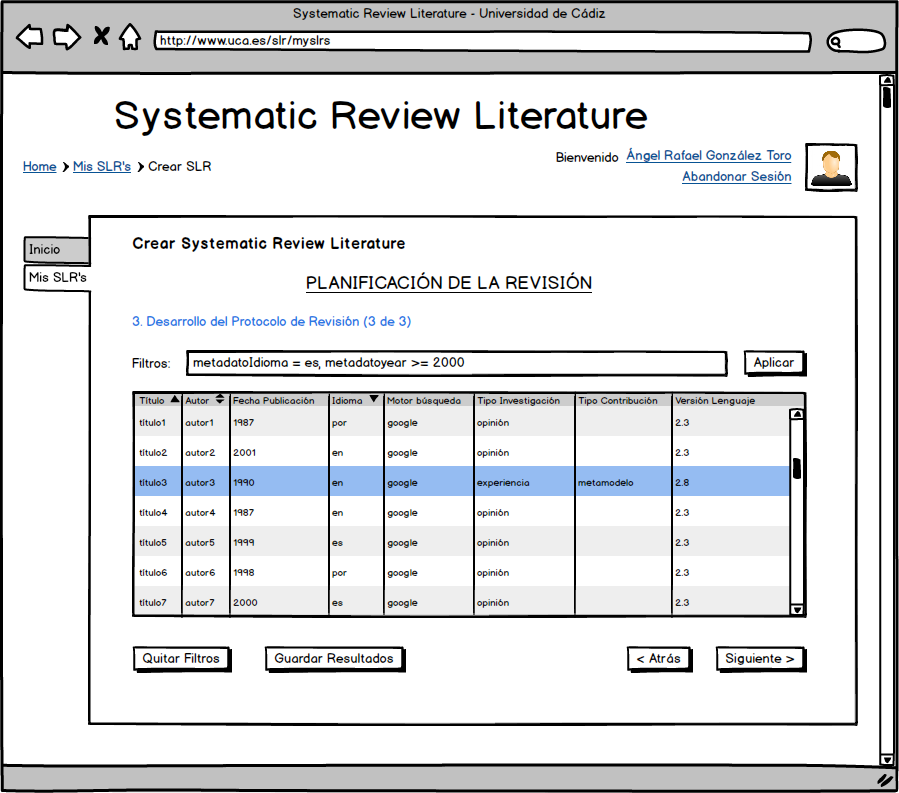
\includegraphics[scale=0.3]{mock07.png}
		\caption{Pantalla Referencias bibliográficas.}
		\label{fig:mock07}
	\end{center}
\end{figure}

\begin{figure}[!hp]
	\begin{center} 
		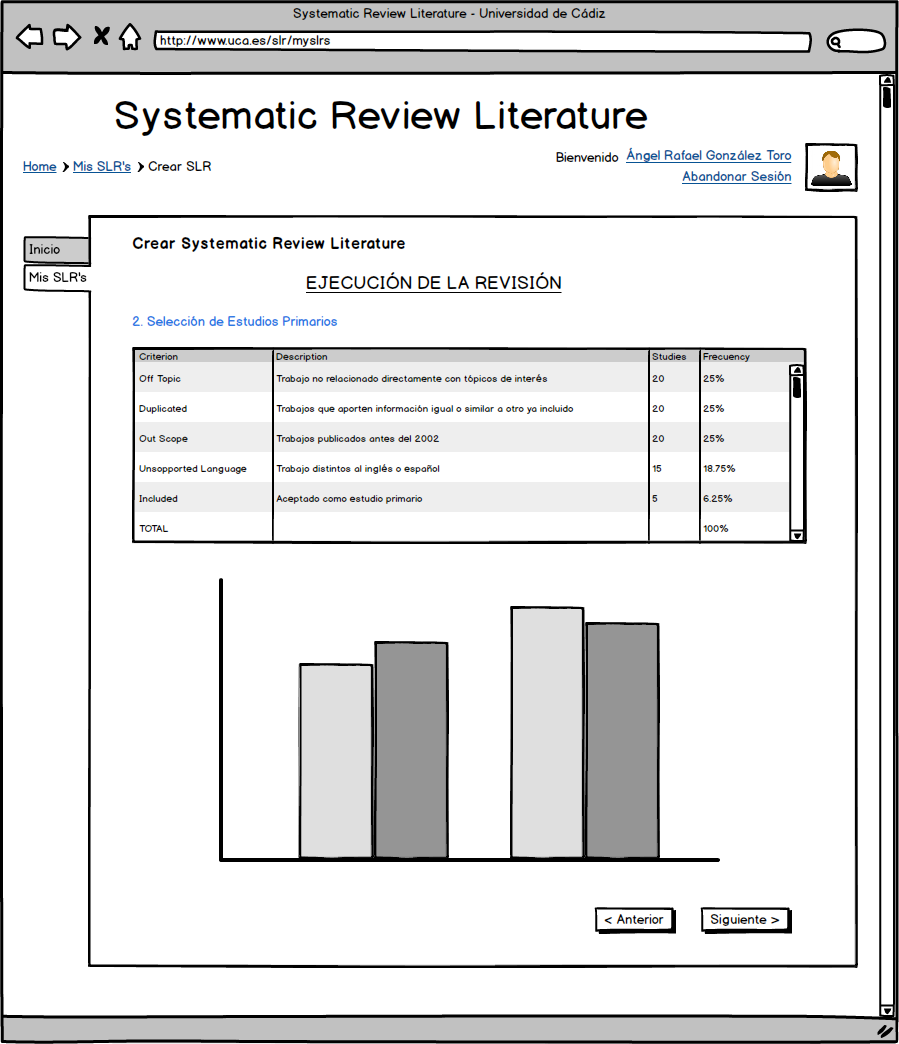
\includegraphics[scale=0.3]{mock08.png}
		\caption{Pantalla exportación referencias bibliográficas y gráficos (I).}
		\label{fig:mock08}
	\end{center}
\end{figure}

\begin{figure}[!hp]
	\begin{center} 
		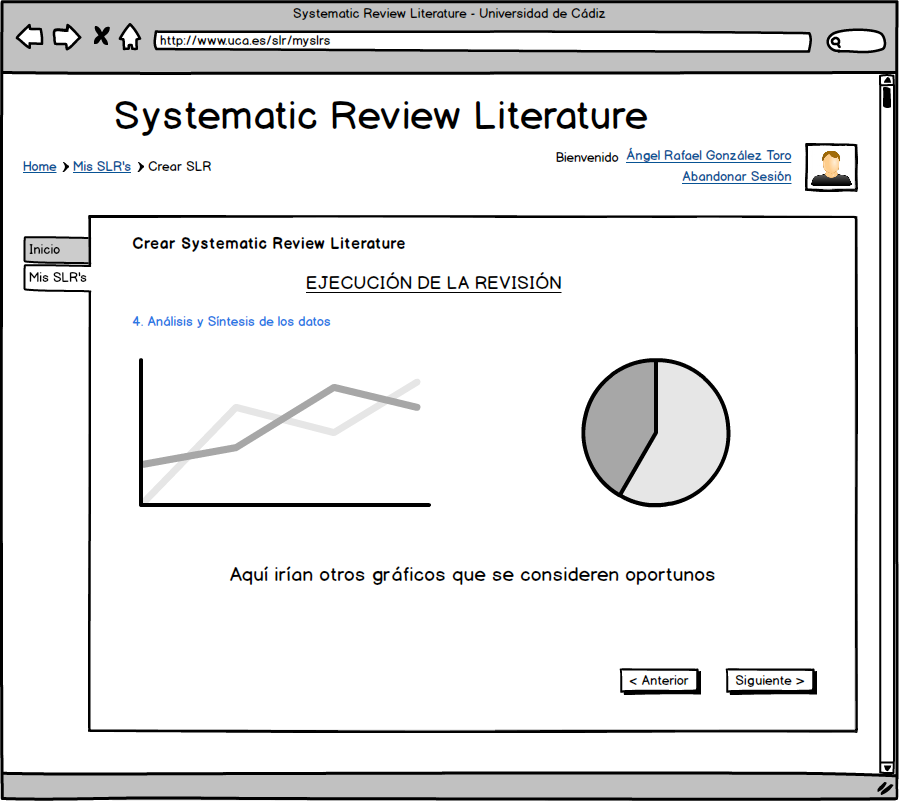
\includegraphics[scale=0.3]{mock09.png}
		\caption{Pantalla exportación referencias bibliográficas y gráficos (II).}
		\label{fig:mock09}
	\end{center}
\end{figure}

%En esta sección se deberá incluir un prototipo de baja fidelidad o mockup de la interfaz de usuario del sistema. Además, es preciso elaborar un diagrama de navegación, reflejando la secuencia de pantallas a las que tienen acceso los diferentes roles de usuario y la conexión entre éstas.


\chapter{Diseño del Sistema}
\label{chap:chap05}
% ------------------------------------------------------------------------------
% Este fichero es parte de la plantilla LaTeX para la realización de Proyectos
% Final de Grado, protegido bajo los términos de la licencia GFDL.
% Para más información, la licencia completa viene incluida en el
% fichero fdl-1.3.tex

% Copyright (C) 2012 SPI-FM. Universidad de Cádiz
% ------------------------------------------------------------------------------

%En esta sección se recoge la arquitectura general del sistema de información, la parametrización del software base (opcional), el diseño físico de datos, el diseño detallado de componentes software y el diseño detallado de la interfaz de usuario.
En esta sección se recoge la arquitectura general del sistema de información, la parametrización del software base, el diseño físico de datos, el diseño detallado de componentes software y el diseño detallado de la interfaz de usuario.

%5.1
\section{Arquitectura del Sistema}
%En esta sección se define la arquitectura general del sistema de información, especificando la infraestructura tecnológica necesaria para dar soporte al software y la estructura de los componentes que lo forman.
En esta sección definiremos la arquitectura general del sistema de información, especificando la infraestructura tecnológica necesaria para dar soporte al software y la estructura de los componentes que lo forman.


%5.1.1
\subsection{Arquitectura Física}
%En este apartado, describimos los principales elementos hardware que forman la arquitectura física de nuestro sistema, recogiendo por un lado los componentes del entorno de producción y los componentes de cliente.\\

%Se debe incluir un modelo de despliegue en el cual se describe cómo los elementos software son desplegados en los elementos hardware. También se incluyen las especificaciones y los requisitos del hardware (servidores, etc.), así como de los elementos software (sistemas operativos, servicios, aplicaciones, etc.) necesarios.
Los componentes que compondrán la arquitectura física de esta aplicación se puede ver reflejado en las figura \ref{fig:arquitectura-fisica01} y \ref{fig:arquitectura-fisica02}.

\begin{itemize}
	\item \textbf{Navegador del cliente}. Un navegador estándar HTML capaz de soportar  CSS, Javascript + Document Object Model, XML y XSLT. Este servirá como dispositivo de interfaz de usuario. Toda la interacción entre los usuarios y el sistema se realiza a través del navegador.
	\item \textbf{Servidor web}. El navegador del cliente accederá al sistema a través del servidor Web (Tomcat), el cual acepta las peticiones del cliente y ejecuta, tosi es necesario, los scripts del lado del servidor necesarios. El resultado, una página HTML formateada, será enviada al cliente.
	\item \textbf{Conexión HTTP}. Es el protocolo más común actualmente entre el cliente y el servidor.
	\item \textbf{Servidor de Aplicaciones}. Es el principal motor para ejecutar la lógica del negocio del lado del servidor.
	\item \textbf{Servidor de Base de datos}. Es la parte del sistema que mantiene el estado actual del negocio.
	\item \textbf{Servicio Web}. En este caso, Mendeley actuará de gestor de referencias del cuál podremos obtener la información de las revisiones sistemáticas (carpetas), ficheros (referencias) e información del perfil del usuario.
\end{itemize}

\begin{figure}[!hp]
	\begin{center} 
		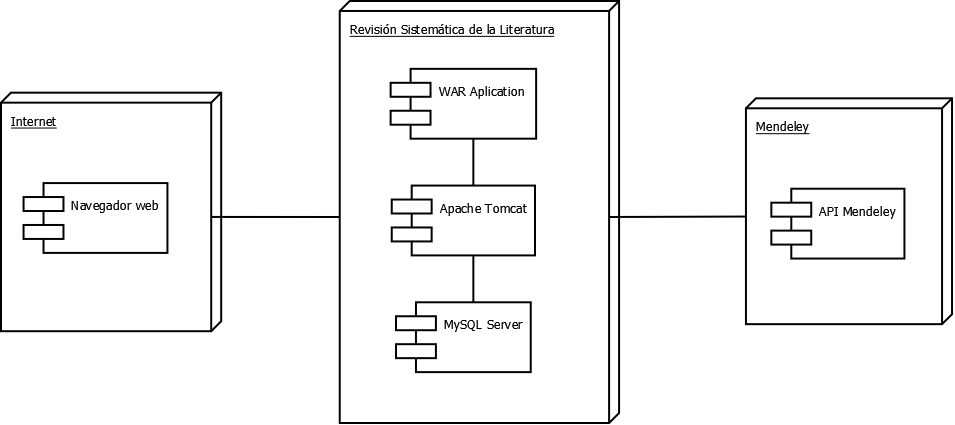
\includegraphics[scale=0.3]{arquitectura-fisica.png}
		\caption{Arquitectura física del sistema (I).}
		\label{fig:arquitectura-fisica01}
	\end{center}
\end{figure}

\begin{figure}[!hp]
	\begin{center} 
		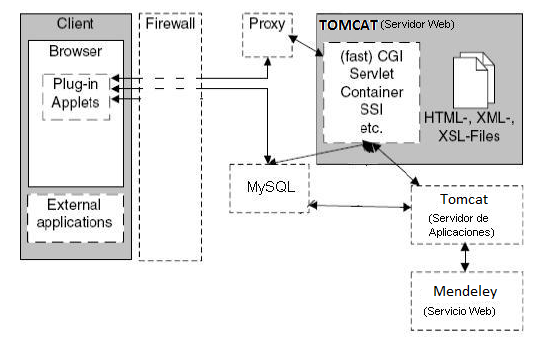
\includegraphics[scale=0.9]{arquitectura-fisica2.png}
		\caption{Arquitectura del sistema (II).}
		\label{fig:arquitectura-fisica02}
	\end{center}
\end{figure}

El servidor tiene las características descritas en la tabla \ref{table:arqui-server}. En él, se ha instalado Tomcat, Apache y MySQL para la base de datos.

\begin{table}[!hbt]
	\begin{center}
		\begin{tabular}{|p{4cm}|p{11cm}|}
			\hline
			\textbf{CPU} & 1vCore\\
			\hline
			\textbf{RAM} & 2048 MB.\\
			\hline
			\textbf{Storage} & 40 GB SSD.\\
			\hline
			\textbf{Bandwidth} & 2000 GB\\
			\hline
		\end{tabular}
		\caption{Arquitectura del Servidor}
		\label{table:arqui-server}
	\end{center}
\end{table}

%5.1.2
\subsection{Arquitectura Lógica}
%La arquitectura de diseño especifica la forma en que los artefactos software interactúan entre sí para lograr el comportamiento deseado en el sistema. En esta sección se muestra la comunicación entre el software base seleccionado, los componentes reutilizados y los componentes desarrollados para cumplir los requisitos de la aplicación. También, se recogen los servicios de sistemas externos con los que interactúa nuestro sistema.
%Se debe incluir un diagrama de componentes que muestre en un alto nivel de abstracción los artefactos que conforman el sistema.\\

%Existen diferentes patrones o estilos arquitectónicos. En los sistemas web de información es común la utilización del patrón Layers (Capas), con el cual estructuramos el sistema en un número apropiado de capas, de forma que todos los componentes de una misma capa trabajan en el mismo nivel de abstracción y los servicios proporcionados por la capa superior utilizan internamente los servicios proporcionados por la capa inmediatamente inferior. Habitualmente se tienen las siguientes capas:

La arquitectura lógica de la aplicación web se va a regir en todo momento según el patrón \textbf{Modelo Vista Controlador} (\textbf{MVC}). Éste separa los datos de la planificación, la interfaz del usuario y la lógica de control o negocio en tres modelos distintos.

\begin{itemize}
	\item \textbf{Capas de datos}. Contiene los componentes que representan y gestionan los datos manejados por la aplicación. En el caso más típico, los objetos encargados de leer y escribir en base de datos.
	\item \textbf{Capa de presentación}. Los componentes de esta capa son responsables de mostrar al usuario el estado actual del modelo de datos, y presentarle las distintas acciones disponibles.
	\item \textbf{Capa de control}. Contendrá todos los componentes que reciban las órdenes del usuario, gestionan la aplicación de la lógica de negocio sobre el modelo de datos, y determinan qué vista debe mostrarse a continuación.
	\item \textbf{Capa de servicios}. Se trata de una cuarta capa que contiene los elementos encargados de implementar la lógica de negocio de nuestra aplicación.
\end{itemize}

Para el desarrollo de la aplicación, se ha decidido seguir la arquitectura del framework \textbf{Grails} (ver figura \ref{fig:arquitectura-grails}) que acopla correctamente el patrón MVC \cite{brito2009}.

\begin{figure}[!hp]
	\begin{center} 
		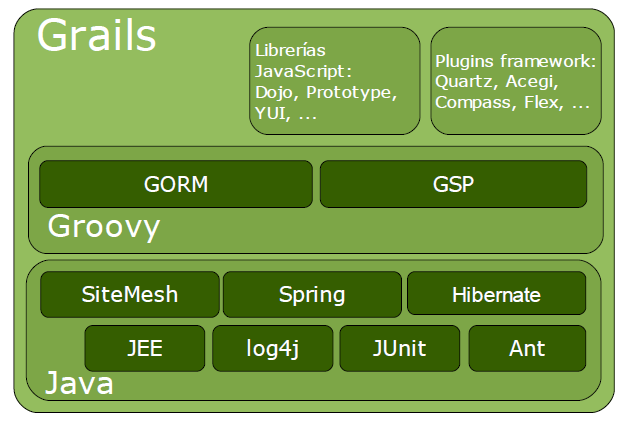
\includegraphics[scale=0.7]{arquitectura-grails.png}
		\caption{Arquitectura Grails.}
		\label{fig:arquitectura-grails}
	\end{center}
\end{figure}

\begin{itemize}
	\item \textbf{Modelo}. Es la representación específica de la información con la cual el sistema opera. La lógica de datos asegura la integridad de éstos. El SGBD para gestionar los datos corresponde a este componente. En este sistema el mapeo se realiza a través de \textbf{GORM} (\textit{Grails Object-Relational Mapping}) que a través de clases escritas en \textbf{Groovy} describe todo el modelo de la aplicación.
	\item \textbf{Vista}. Presenta el modelo en un formato adecuado para interactuar, normalmente la interfaz de usuario. La vista estará formada por un conjunto de páginas webs que facilitaran al usuario la interacción con el sistema. Las páginas se renderizan a partir de ficheros fuentes GSP (Groovy Server Pages) que mezcla etiquetas HTML con otras propias de Grails.
	\item \textbf{Controlador}. Responde a los eventos, generalmente provocados por el usuario a través de las vistas, ajustando los modelos. Estos controladores serán clases escritas en Groovy con cada una de las acciones posibles.
\end{itemize}

Grails es un framework para desarrollo de aplicaciones web construido sobre cinco fuertes pilares:

\begin{itemize}
	\item Groovy. Para la creación de propiedades y métodos dinámicos en los objetos de la aplicación.
	\item Spring. Para los flujos de trabajo e inyección de dependencias.
	\item Hibernate. Para la persistencia de los datos de la aplicación.
	\item SiteMesh. Para la composición de la vista.
	\item Ant. Para la gestión del proceso de desarrollo.
\end{itemize}

La estructura de esta aplicación será la siguiente:

\begin{itemize}
	\item grails-app
\begin{itemize}
	\item conf: Archivos de configuración.
	\item hibernate: Configuración de Hibernate.
	\item spring: Configuración de Spring.
	\item controllers: Controladores.
	\item domain: Entidades (Clases de Dominio).
	\item i18n: Message Bundles.
	\item services: Servicios.
	\item taglib: Librerías de etiquetas.
	\item util: Clases de utilidad.
	\item views: Vistas.
	\item layouts: Layouts SiteMesh.
	\item lib
	\item scripts
	\item src
	\begin{itemize}
		\item groovy: Clases Groovy.
		\item java: Clases Java.
	\end{itemize}
	\item test: Casos de prueba.
	\item web-app: Raíz de la aplicación web.
	\end{itemize}
\end{itemize}

%\paragraph*{Capa de presentación (frontend)}
%Este grupo de artefactos software conforman la capa de presentación del sistema, incluyendo tanto los componentes de la vista como los elementos de control de la misma.

%\paragraph*{Capa de negocio}
%Este grupo de artefactos software conforman la capa de negocio del sistema, incluyendo los elementos del modelo de dominio y los servicios (operaciones del sistema).

%\paragraph*{Capa de persistencia}
%Este grupo de artefactos software conforman la capa de integración del sistema, incluyendo las clases de abstracción para el acceso a datos (BD o sistema de ficheros) o a sistemas heredados.\\

%Es común que a la capa de negocio y de datos de los sistemas web, se denomine conjuntamente como backend o modelo de la aplicación.

%Opcionalmente, podemos disponer de un conjunto de artefactos software que pueden ser usados por elementos de cualquiera de las capas del sistema y que fundamentalmente proporcionan servicios relacionados con requisitos no funcionales (calidad).

%5.2
\section{Parametrización del software base}
%En esta sección, se detallan las modificaciones a realizar sobre el software base, que son requeridas para la correcta construcción del sistema. En esta sección incluiremos las  actuaciones necesarias sobre la interfaz de administración del sistema, sobre el código fuente o sobre el modelo de datos.
Esta aplicación hace conexión a través de una API al gestor de referencias Mendeley. Para realizar este proceso, se necesita un usuario que actue como administrador del sistema y que se conecte con sus datos al portal de Mendeley para indicar que esta aplicación pueda tener conexión con Mendeley.\\

Mendeley, dispone de una sección donde todos los usuarios pueden insertar la configuración necesaria para que Mendeley conecte con sus aplicaciones. Para ello, es necesario dirigirse a \url{http://dev.mendeley.com/} y a continuación elegir la opción \textit{My Apps}.\\

Una vez que se ha logado en el sistema, podemos obtener un listado de aplicaciones (ver figura \ref{fig:mend-register}) con todas las aplicaciones que un usuario disponga. Mendeley pide por pantalla varios datos de configuración, pero es necesario recordar tres campos que serán necesarios para la configuración en nuestra aplicación como describiremos más adelante (marcados en negrita). Como podemos comprobar, se puede tener tantas configuraciones como se desee. Ésto podrá ser válido si, por ejemplo, tuviésemos varios entornos de desarrollo.

\begin{itemize}
	\item Application name. Nombre de la aplicación.
	\item Description. Descripción de lo que realiza esta aplicación.
	\item \textbf{ID Cliente}. Identificador de esta aplicación en Mendeley. Es generado automáticamente por Mendeley.
	\item \textbf{Redirect URL}. Esta aplicación hará conexión con Mendeley a través de OAuth2, donde se nos pedirá unos datos que enviarán a una página de nuestra aplicación. 
	\item \textbf{Client Secret}. Código privado del cliente que debe ser generado a través del botón \textit{Generate secret}.
\end{itemize}

\begin{figure}[!hp]
	\begin{center} 
		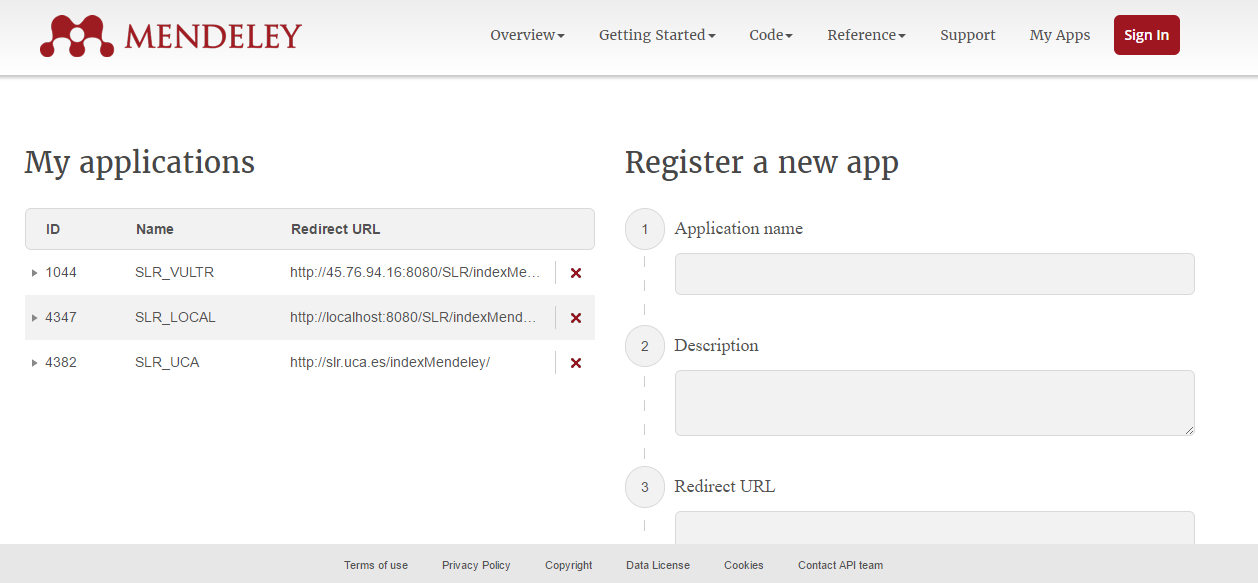
\includegraphics[scale=0.4]{mendeley-registerApp.png}
		\caption{Registrar aplicación en Mendeley.}
		\label{fig:mend-register}
	\end{center}
\end{figure}

Una vez que hemos realizado la configuración en Mendeley, debemos insertar la información obtenida en nuestra aplicación. Para ello, Grails dispone de un fichero situado en \textit{conf/Bootstrap.groovy} donde por medio de una clase de dominio realizada denominada \textit{MendeleyApi} podemos parametrizar esta configuración tal y como podemos ver reflejado en la figura \ref{fig:bootstrap-mend}.

\begin{figure}[!hp]
	\begin{center} 
		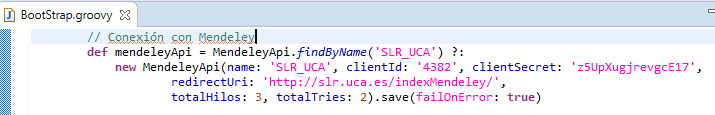
\includegraphics[scale=0.6]{bootstrap-mend.png}
		\caption{Registrar aplicación en Mendeley.}
		\label{fig:bootstrap-mend}
	\end{center}
\end{figure}

Si la aplicación se encuentra desplegada sobre el servidor, y siempre siendo administrador, podemos modificar esta configuración a través de un menú que dispone un usuario con este rol.

%5.3
\section{Diseño Físico de Datos}
En esta sección se define la estructura física de datos que utilizará el sistema, a partir del modelo de conceptual de clases, de manera que teniendo presente los requisitos establecidos para el sistema de información y las particularidades del entorno tecnológico, se consiga un acceso eficiente de los datos.
La estructura física se compone de tablas, índices, procedimientos almacenados, secuencias y otros elementos dependientes del SGBD a utilizar.

%5.4
\section{Diseño detallado de Componentes}
Para cada uno de los módulos funcionales del sistema debemos realizar un diagrama de secuencia, para definir la interacción existente entre las clases de objetos que permitan responder a eventos externos.

%5.5
\section{Diseño detallado de la Interfaz de Usuario} 
En esta sección se detallarán las interfaces entre el sistema y el usuario, incluyendo un prototipo de alta fidelidad con el diseño de la IU. Se definirá el comportamiento de las diferentes pantallas, indicando qué ocurre en los distintos componentes visuales de la interfaz cuando aparecen y qué acciones se disparan cuando el usuario trabaja con ellas.



\chapter{Construcción del Sistema}
\label{chap:chap06}
% ------------------------------------------------------------------------------
% Este fichero es parte de la plantilla LaTeX para la realización de Proyectos
% Final de Grado, protegido bajo los términos de la licencia GFDL.
% Para más información, la licencia completa viene incluida en el
% fichero fdl-1.3.tex

% Copyright (C) 2012 SPI-FM. Universidad de Cádiz
% ------------------------------------------------------------------------------

Este capítulo trata sobre todos los aspectos relacionados con la implementación del sistema en código, haciendo uso de un determinado entorno tecnológico.

\section{Entorno de Construcción}
En esta sección se debe indicar el marco tecnológico utilizado para la construcción del sistema: entorno de desarrollo (IDE), lenguaje de programación, herramientas de ayuda a la construcción y despliegue, control de versiones, repositorio de componentes, integración contínua, etc.

\section{Código Fuente}
Organización del código fuente, describiendo la utilidad de los diferentes ficheros y su distribución en paquetes o directorios. Asimismo, se incluirá algún extracto significativo de código fuente que sea de interés para ilustrar algún algoritmo o funcionalidad específica del sistema.

\section{Scripts de Base de datos}
Organización del código fuente, describiendo la utilidad de los diferentes ficheros y su distribución en paquetes o directorios. Asimismo, se incluirá el script de algún disparador o un procedimiento almacenado, que sea de interés para ilustrar algún aspecto concreto de la gestión de la base de datos.


\chapter{Pruebas del Sistema}
\label{chap:chap07}
% ------------------------------------------------------------------------------
% Este fichero es parte de la plantilla LaTeX para la realización de Proyectos
% Final de Grado, protegido bajo los términos de la licencia GFDL.
% Para más información, la licencia completa viene incluida en el
% fichero fdl-1.3.tex

% Copyright (C) 2012 SPI-FM. Universidad de Cádiz
% ------------------------------------------------------------------------------

En este capítulo se presenta el plan de pruebas del sistema de información, incluyendo los diferentes tipos de pruebas que se han llevado a cabo, ya sean manuales (mediante listas de comprobación) o automatizadas mediante algún software específico de pruebas.

\section{Estrategia}
En esta sección se debe incluir el alcance de las pruebas, hasta donde se pretende llegar con ellas, si se registrarán todas o sólo aquellas de un cierto tipo y cómo se interpretarán y evaluarán los resultados.
También, se incluirá el procedimiento a seguir para las pruebas de regresión, esto es, la repetición de ciertas pruebas para comprobar que nuevos cambios que se vayan introduciendo no originen errores en el software ya probado.

\section{Entorno de Pruebas}
Incluir en este apartado los requisitos de los entornos hardware/software donde se ejecutarán las pruebas.

\section{Roles}
Describir en esa sección cuáles serán los perfiles y participantes necesarios para la ejecución de cada uno de los niveles de prueba.

\section{Niveles de Pruebas}
En este sección se documentan los diferentes tipos de pruebas que se han llevado a cabo, ya sean manuales o automatizadas mediante algún software específico de pruebas.

\subsection{Pruebas Unitarias}
Las pruebas unitarias tienen por objetivo localizar errores en cada nuevo artefacto software desarrollado, antes que se produzca la integración con el resto de artefactos del sistema.

\subsection{Pruebas de Integración}
Este tipo de pruebas tienen por objetivo localizar errores en módulos o subsistemas completos, analizando la interacción entre varios artefactos software.

\subsection{Pruebas de Sistema}
En esta actividad se realizan las pruebas de sistema de modo que se asegure que el sistema cumple con todos los requisitos establecidos: funcionales, de almacenamiento, reglas de negocio y no funcionales. Se suelen desarrollar en un entorno específico para pruebas.

\subsubsection{Pruebas Funcionales}
Con estas pruebas se analiza el buen funcionamiento de la implementación de los flujos normales y alternativos de los distintos casos de uso del sistema.

\subsubsection{Pruebas No Funcionales}
Estas pruebas pretenden comprobar el funcionamiento del sistema, con respecto a los requisitos no funcionales identificados: eficiencia, seguridad, etc.

\subsection{Pruebas de Aceptación}
El objetivo de estas pruebas es demostrar que el producto está listo para el paso a producción. Suelen ser las mismas pruebas que se realizaron anteriormente pero en el entorno de producción. En estas pruebas, es importante la participación del cliente final.

% EPILOGO
\part{Epílogo}
\null\vfill
\noindent En esta última parte quedarán recogidas las conclusiones y los manuales necesarios para el manejo de la aplicación resultado del desarrollo. Si se ha realizado algún tipo de evaluación de la solución proporcionada, más allá de las pruebas del sistema, también deberá venir recogida en un capítulo separado dentro de esta parte. Pueden consultarse diversos tipos de evaluaciones sobre sistemas de información en \cite{hevner2004}: casos de estudio, análisis estático, análisis dinámico, simulación, experimento controlado, etc.
\vfill

\chapter{Manual de implantación y explotación}
\label{chap:chap08}
% ------------------------------------------------------------------------------
% Este fichero es parte de la plantilla LaTeX para la realización de Proyectos
% Final de Grado, protegido bajo los términos de la licencia GFDL.
% Para más información, la licencia completa viene incluida en el
% fichero fdl-1.3.tex

% Copyright (C) 2012 SPI-FM. Universidad de Cádiz
% ------------------------------------------------------------------------------

Las instrucciones de instalación y explotación del sistema se detallan a continuación. Este manual resulta de aplicación en aquellos casos en que se requiere realizar la instalación del software objetivo de este proyecto sobre algún entorno de servidor o cuando su instalación no sea trivial.

\section{Introducción}
Resumen de los principales objetivos, ámbito, características y alcance del software desarrollado.

\section{Requisitos previos}
Requisitos hardware y software para la correcta instalación del sistema.

\section{Inventario de componentes}
Lista de los componentes hardware y software que se incluyen en la versión del producto.

\section{Procedimientos de instalación}
Procedimientos de instalación y configuración de cada componente hardware y software (base y desarrollado) para asegurar la correcta instalación y explotación del sistema, así como aquellos procedimientos necesarios de migración/carga de datos.

\section{Pruebas de implantación}
Descripción de las pruebas a realizar después de la instalación del sistema. 

\section{Procedimientos de operación y nivel de servicio}
Procedimientos necesarios para asegurar el correcto funcionamiento, rendimiento, disponibilidad y seguridad del sistema: back-ups, chequeo de logs, etc. También, es preciso indicar claramente aquellas actuaciones precisas necesarias para el mantenimiento preventivo del sistema y así prevenir posibles fallos en el mismo. 


\chapter{Manual de usuario}
\label{chap:chap09}
% ------------------------------------------------------------------------------
% Este fichero es parte de la plantilla LaTeX para la realización de Proyectos
% Final de Grado, protegido bajo los términos de la licencia GFDL.
% Para más información, la licencia completa viene incluida en el
% fichero fdl-1.3.tex

% Copyright (C) 2012 SPI-FM. Universidad de Cádiz
% ------------------------------------------------------------------------------

Las instrucciones de uso del software se detallan a continuación. Este manual se dirige al usuario final del software objetivo de este proyecto.

\section{Introducción}
Resumen de los principales objetivos, ámbito, características y alcance del software desarrollado.

\section{Instalación}
Se detallarán los pasos necesarios para la obtención e instalación del software, así como los requisitos previos de hardware y software.

\section{Uso del sistema}
Describir todos los aspectos necesarios para una utilización efectiva y eficiente de las características del sistema por parte de los usuarios.





\chapter{Manual del desarrollador}
\label{chap:chap10}
% ------------------------------------------------------------------------------
% Este fichero es parte de la plantilla LaTeX para la realización de Proyectos
% Final de Grado, protegido bajo los términos de la licencia GFDL.
% Para más información, la licencia completa viene incluida en el
% fichero fdl-1.3.tex

% Copyright (C) 2012 SPI-FM. Universidad de Cádiz
% ------------------------------------------------------------------------------

A continuación se recogen las instrucciones necesarias para evolucionar el software. Este manual está dirigido a los desarrolladores que pretenden extender o modificar el código fuente, con el fin de incorporar nuevas funcionalidades o modificar las ya existentes. A lo largo de este capítulo se deberán hacer referencias explicitas a aquellos epígrafes de los capítulos de Diseño, Construcción y Pruebas del Sistema que resulten de interés.

\section{Introducción}
Resumen de los principales objetivos, ámbito, características y alcance del software desarrollado.

\section{Preparación del entorno de trabajo}
Descripción de los requisitos (hardware y software) previos. Datos de interés relativos al control de versiones del software. Detalles sobre la instalación en local del entorno de desarrollo y, si fuesen necesarios, de otros componentes como bases de datos, servidores de aplicaciones, etc. 

\section{Consideraciones generales sobre el desarrollo}
Aspectos importantes a tener en cuenta a la hora de modificar y extender el código fuente, guías de estilo, etc. Asimismo, se detallarán las directrices que sean de aplicación a la hora de realizar pruebas sobre las nuevas mejoras introducidas.

\section{Instrucciones para construcción y despliegue}
Secuencia de pasos requeridos para llevar a cabo la compilación del código fuente y así poder construir y depurar el software sobre una máquina de desarrollo.


\chapter{Conclusiones}
\label{chap:chap11}
% ------------------------------------------------------------------------------
% Este fichero es parte de la plantilla LaTeX para la realización de Proyectos
% Final de Grado, protegido bajo los términos de la licencia GFDL.
% Para más información, la licencia completa viene incluida en el
% fichero fdl-1.3.tex

% Copyright (C) 2012 SPI-FM. Universidad de Cádiz
% ------------------------------------------------------------------------------

En este último capítulo se detallan las lecciones aprendidas tras el desarrollo del presente proyecto y se identifican las posibles oportunidades de mejora sobre el software desarrollado.

\section{Objetivos alcanzados}
Este apartado debe resumir los objetivos generales y específicos alcanzados, relacionándolos con todo lo descrito en el capítulo de introducción.\\

\section{Lecciones aprendidas}
A continuación, se detallan las buenas prácticas adquiridas, tanto tecnológicas como procedimentales, así como cualquier otro aspecto de interés.\\
Resumir cuantitativamente el tiempo y esfuerzo dedicados al proyecto a lo largo de su desarrollo que escribir un sencillo 'he trabajado mucho en este proyecto'.

\section{Trabajo futuro}
En esta sección, se presentan las diversas áreas u oportunidades de mejora detectadas durante el desarrollo del proyecto y que podrán ser abarcadas en futuras versiones del software.\\

Los elementos aquí descritos deben estar en relación con lo relatado en el apartado de objetivos y alcance del proyecto descritos en la introducción.



\chapter*{\bibname}
\addcontentsline{toc}{chapter}{\bibname}
%\renewcommand{\bibname}{}

%\input{./bibliografia}

\begingroup
  \def\chapter*#1{}
\renewcommand{\bibname}{}
% Bibliografía con BibTeX
\bibliographystyle{apalike}
\bibliography{bibliografia}

\backmatter

% ------------------------------------------------------------------------------
% Este fichero es parte de la plantilla LaTeX para la realización de Proyectos
% Final de Grado, protegido bajo los términos de la licencia GFDL.
% Para más información, la licencia completa viene incluida en el
% fichero fdl-1.3.tex

% Copyright (C) 2012 SPI-FM. Universidad de Cádiz
% ------------------------------------------------------------------------------


\chapter*{\rlap{Información sobre Licencia}}
\phantomsection  % so hyperref creates bookmarks
\addcontentsline{toc}{chapter}{Información sobre Licencia}
%\label{label_fdl}

 \begin{center}

       Información sobre Licencia


\end{center}

Incluir aquí la información relativa a la licencia seleccionada para la documentación y software del presente proyecto.

%GNU % ------------------------------------------------------------------------------
% Este fichero es parte de la plantilla LaTeX para la realización de Proyectos
% Final de Grado, protegido bajo los términos de la licencia GFDL.
% Para más información, la licencia completa viene incluida en el
% fichero fdl-1.3.tex

% Copyright (C) 2012 SPI-FM. Universidad de Cádiz
% ------------------------------------------------------------------------------


\chapter*{\rlap{GNU Free Documentation License}}
\phantomsection  % so hyperref creates bookmarks
\addcontentsline{toc}{chapter}{GNU Free Documentation License}
%\label{label_fdl}

 \begin{center}

       Version 1.3, 3 November 2008


 Copyright \copyright{} 2000, 2001, 2002, 2007, 2008  Free Software Foundation, Inc.
 
 \bigskip
 
     <http://fsf.org/>
  
 \bigskip
 
 Everyone is permitted to copy and distribute verbatim copies
 of this license document, but changing it is not allowed.
\end{center}


\begin{center}
{\bf\large Preamble}
\end{center}

The purpose of this License is to make a manual, textbook, or other
functional and useful document ``free'' in the sense of freedom: to
assure everyone the effective freedom to copy and redistribute it,
with or without modifying it, either commercially or noncommercially.
Secondarily, this License preserves for the author and publisher a way
to get credit for their work, while not being considered responsible
for modifications made by others.

This License is a kind of ``copyleft'', which means that derivative
works of the document must themselves be free in the same sense.  It
complements the GNU General Public License, which is a copyleft
license designed for free software.

We have designed this License in order to use it for manuals for free
software, because free software needs free documentation: a free
program should come with manuals providing the same freedoms that the
software does.  But this License is not limited to software manuals;
it can be used for any textual work, regardless of subject matter or
whether it is published as a printed book.  We recommend this License
principally for works whose purpose is instruction or reference.


\begin{center}
{\Large\bf 1. APPLICABILITY AND DEFINITIONS\par}
\phantomsection
\addcontentsline{toc}{section}{1. APPLICABILITY AND DEFINITIONS}
\end{center}

This License applies to any manual or other work, in any medium, that
contains a notice placed by the copyright holder saying it can be
distributed under the terms of this License.  Such a notice grants a
world-wide, royalty-free license, unlimited in duration, to use that
work under the conditions stated herein.  The ``\textbf{Document}'', below,
refers to any such manual or work.  Any member of the public is a
licensee, and is addressed as ``\textbf{you}''.  You accept the license if you
copy, modify or distribute the work in a way requiring permission
under copyright law.

A ``\textbf{Modified Version}'' of the Document means any work containing the
Document or a portion of it, either copied verbatim, or with
modifications and/or translated into another language.

A ``\textbf{Secondary Section}'' is a named appendix or a front-matter section of
the Document that deals exclusively with the relationship of the
publishers or authors of the Document to the Document's overall subject
(or to related matters) and contains nothing that could fall directly
within that overall subject.  (Thus, if the Document is in part a
textbook of mathematics, a Secondary Section may not explain any
mathematics.)  The relationship could be a matter of historical
connection with the subject or with related matters, or of legal,
commercial, philosophical, ethical or political position regarding
them.

The ``\textbf{Invariant Sections}'' are certain Secondary Sections whose titles
are designated, as being those of Invariant Sections, in the notice
that says that the Document is released under this License.  If a
section does not fit the above definition of Secondary then it is not
allowed to be designated as Invariant.  The Document may contain zero
Invariant Sections.  If the Document does not identify any Invariant
Sections then there are none.

The ``\textbf{Cover Texts}'' are certain short passages of text that are listed,
as Front-Cover Texts or Back-Cover Texts, in the notice that says that
the Document is released under this License.  A Front-Cover Text may
be at most 5 words, and a Back-Cover Text may be at most 25 words.

A ``\textbf{Transparent}'' copy of the Document means a machine-readable copy,
represented in a format whose specification is available to the
general public, that is suitable for revising the document
straightforwardly with generic text editors or (for images composed of
pixels) generic paint programs or (for drawings) some widely available
drawing editor, and that is suitable for input to text formatters or
for automatic translation to a variety of formats suitable for input
to text formatters.  A copy made in an otherwise Transparent file
format whose markup, or absence of markup, has been arranged to thwart
or discourage subsequent modification by readers is not Transparent.
An image format is not Transparent if used for any substantial amount
of text.  A copy that is not ``Transparent'' is called ``\textbf{Opaque}''.

Examples of suitable formats for Transparent copies include plain
ASCII without markup, Texinfo input format, LaTeX input format, SGML
or XML using a publicly available DTD, and standard-conforming simple
HTML, PostScript or PDF designed for human modification.  Examples of
transparent image formats include PNG, XCF and JPG.  Opaque formats
include proprietary formats that can be read and edited only by
proprietary word processors, SGML or XML for which the DTD and/or
processing tools are not generally available, and the
machine-generated HTML, PostScript or PDF produced by some word
processors for output purposes only.

The ``\textbf{Title Page}'' means, for a printed book, the title page itself,
plus such following pages as are needed to hold, legibly, the material
this License requires to appear in the title page.  For works in
formats which do not have any title page as such, ``Title Page'' means
the text near the most prominent appearance of the work's title,
preceding the beginning of the body of the text.

The ``\textbf{publisher}'' means any person or entity that distributes
copies of the Document to the public.

A section ``\textbf{Entitled XYZ}'' means a named subunit of the Document whose
title either is precisely XYZ or contains XYZ in parentheses following
text that translates XYZ in another language.  (Here XYZ stands for a
specific section name mentioned below, such as ``\textbf{Acknowledgements}'',
``\textbf{Dedications}'', ``\textbf{Endorsements}'', or ``\textbf{History}''.)  
To ``\textbf{Preserve the Title}''
of such a section when you modify the Document means that it remains a
section ``Entitled XYZ'' according to this definition.

The Document may include Warranty Disclaimers next to the notice which
states that this License applies to the Document.  These Warranty
Disclaimers are considered to be included by reference in this
License, but only as regards disclaiming warranties: any other
implication that these Warranty Disclaimers may have is void and has
no effect on the meaning of this License.


\begin{center}
{\Large\bf 2. VERBATIM COPYING\par}
\phantomsection
\addcontentsline{toc}{section}{2. VERBATIM COPYING}
\end{center}

You may copy and distribute the Document in any medium, either
commercially or noncommercially, provided that this License, the
copyright notices, and the license notice saying this License applies
to the Document are reproduced in all copies, and that you add no other
conditions whatsoever to those of this License.  You may not use
technical measures to obstruct or control the reading or further
copying of the copies you make or distribute.  However, you may accept
compensation in exchange for copies.  If you distribute a large enough
number of copies you must also follow the conditions in section~3.

You may also lend copies, under the same conditions stated above, and
you may publicly display copies.


\begin{center}
{\Large\bf 3. COPYING IN QUANTITY\par}
\phantomsection
\addcontentsline{toc}{section}{3. COPYING IN QUANTITY}
\end{center}


If you publish printed copies (or copies in media that commonly have
printed covers) of the Document, numbering more than 100, and the
Document's license notice requires Cover Texts, you must enclose the
copies in covers that carry, clearly and legibly, all these Cover
Texts: Front-Cover Texts on the front cover, and Back-Cover Texts on
the back cover.  Both covers must also clearly and legibly identify
you as the publisher of these copies.  The front cover must present
the full title with all words of the title equally prominent and
visible.  You may add other material on the covers in addition.
Copying with changes limited to the covers, as long as they preserve
the title of the Document and satisfy these conditions, can be treated
as verbatim copying in other respects.

If the required texts for either cover are too voluminous to fit
legibly, you should put the first ones listed (as many as fit
reasonably) on the actual cover, and continue the rest onto adjacent
pages.

If you publish or distribute Opaque copies of the Document numbering
more than 100, you must either include a machine-readable Transparent
copy along with each Opaque copy, or state in or with each Opaque copy
a computer-network location from which the general network-using
public has access to download using public-standard network protocols
a complete Transparent copy of the Document, free of added material.
If you use the latter option, you must take reasonably prudent steps,
when you begin distribution of Opaque copies in quantity, to ensure
that this Transparent copy will remain thus accessible at the stated
location until at least one year after the last time you distribute an
Opaque copy (directly or through your agents or retailers) of that
edition to the public.

It is requested, but not required, that you contact the authors of the
Document well before redistributing any large number of copies, to give
them a chance to provide you with an updated version of the Document.


\begin{center}
{\Large\bf 4. MODIFICATIONS\par}
\phantomsection
\addcontentsline{toc}{section}{4. MODIFICATIONS}
\end{center}

You may copy and distribute a Modified Version of the Document under
the conditions of sections 2 and 3 above, provided that you release
the Modified Version under precisely this License, with the Modified
Version filling the role of the Document, thus licensing distribution
and modification of the Modified Version to whoever possesses a copy
of it.  In addition, you must do these things in the Modified Version:

\begin{itemize}
\item[A.] 
   Use in the Title Page (and on the covers, if any) a title distinct
   from that of the Document, and from those of previous versions
   (which should, if there were any, be listed in the History section
   of the Document).  You may use the same title as a previous version
   if the original publisher of that version gives permission.
   
\item[B.]
   List on the Title Page, as authors, one or more persons or entities
   responsible for authorship of the modifications in the Modified
   Version, together with at least five of the principal authors of the
   Document (all of its principal authors, if it has fewer than five),
   unless they release you from this requirement.
   
\item[C.]
   State on the Title page the name of the publisher of the
   Modified Version, as the publisher.
   
\item[D.]
   Preserve all the copyright notices of the Document.
   
\item[E.]
   Add an appropriate copyright notice for your modifications
   adjacent to the other copyright notices.
   
\item[F.]
   Include, immediately after the copyright notices, a license notice
   giving the public permission to use the Modified Version under the
   terms of this License, in the form shown in the Addendum below.
   
\item[G.]
   Preserve in that license notice the full lists of Invariant Sections
   and required Cover Texts given in the Document's license notice.
   
\item[H.]
   Include an unaltered copy of this License.
   
\item[I.]
   Preserve the section Entitled ``History'', Preserve its Title, and add
   to it an item stating at least the title, year, new authors, and
   publisher of the Modified Version as given on the Title Page.  If
   there is no section Entitled ``History'' in the Document, create one
   stating the title, year, authors, and publisher of the Document as
   given on its Title Page, then add an item describing the Modified
   Version as stated in the previous sentence.
   
\item[J.]
   Preserve the network location, if any, given in the Document for
   public access to a Transparent copy of the Document, and likewise
   the network locations given in the Document for previous versions
   it was based on.  These may be placed in the ``History'' section.
   You may omit a network location for a work that was published at
   least four years before the Document itself, or if the original
   publisher of the version it refers to gives permission.
   
\item[K.]
   For any section Entitled ``Acknowledgements'' or ``Dedications'',
   Preserve the Title of the section, and preserve in the section all
   the substance and tone of each of the contributor acknowledgements
   and/or dedications given therein.
   
\item[L.]
   Preserve all the Invariant Sections of the Document,
   unaltered in their text and in their titles.  Section numbers
   or the equivalent are not considered part of the section titles.
   
\item[M.]
   Delete any section Entitled ``Endorsements''.  Such a section
   may not be included in the Modified Version.
   
\item[N.]
   Do not retitle any existing section to be Entitled ``Endorsements''
   or to conflict in title with any Invariant Section.
   
\item[O.]
   Preserve any Warranty Disclaimers.
\end{itemize}

If the Modified Version includes new front-matter sections or
appendices that qualify as Secondary Sections and contain no material
copied from the Document, you may at your option designate some or all
of these sections as invariant.  To do this, add their titles to the
list of Invariant Sections in the Modified Version's license notice.
These titles must be distinct from any other section titles.

You may add a section Entitled ``Endorsements'', provided it contains
nothing but endorsements of your Modified Version by various
parties---for example, statements of peer review or that the text has
been approved by an organization as the authoritative definition of a
standard.

You may add a passage of up to five words as a Front-Cover Text, and a
passage of up to 25 words as a Back-Cover Text, to the end of the list
of Cover Texts in the Modified Version.  Only one passage of
Front-Cover Text and one of Back-Cover Text may be added by (or
through arrangements made by) any one entity.  If the Document already
includes a cover text for the same cover, previously added by you or
by arrangement made by the same entity you are acting on behalf of,
you may not add another; but you may replace the old one, on explicit
permission from the previous publisher that added the old one.

The author(s) and publisher(s) of the Document do not by this License
give permission to use their names for publicity for or to assert or
imply endorsement of any Modified Version.


\begin{center}
{\Large\bf 5. COMBINING DOCUMENTS\par}
\phantomsection
\addcontentsline{toc}{section}{5. COMBINING DOCUMENTS}
\end{center}


You may combine the Document with other documents released under this
License, under the terms defined in section~4 above for modified
versions, provided that you include in the combination all of the
Invariant Sections of all of the original documents, unmodified, and
list them all as Invariant Sections of your combined work in its
license notice, and that you preserve all their Warranty Disclaimers.

The combined work need only contain one copy of this License, and
multiple identical Invariant Sections may be replaced with a single
copy.  If there are multiple Invariant Sections with the same name but
different contents, make the title of each such section unique by
adding at the end of it, in parentheses, the name of the original
author or publisher of that section if known, or else a unique number.
Make the same adjustment to the section titles in the list of
Invariant Sections in the license notice of the combined work.

In the combination, you must combine any sections Entitled ``History''
in the various original documents, forming one section Entitled
``History''; likewise combine any sections Entitled ``Acknowledgements'',
and any sections Entitled ``Dedications''.  You must delete all sections
Entitled ``Endorsements''.

\begin{center}
{\Large\bf 6. COLLECTIONS OF DOCUMENTS\par}
\phantomsection
\addcontentsline{toc}{section}{6. COLLECTIONS OF DOCUMENTS}
\end{center}

You may make a collection consisting of the Document and other documents
released under this License, and replace the individual copies of this
License in the various documents with a single copy that is included in
the collection, provided that you follow the rules of this License for
verbatim copying of each of the documents in all other respects.

You may extract a single document from such a collection, and distribute
it individually under this License, provided you insert a copy of this
License into the extracted document, and follow this License in all
other respects regarding verbatim copying of that document.


\begin{center}
{\Large\bf 7. AGGREGATION WITH INDEPENDENT WORKS\par}
\phantomsection
\addcontentsline{toc}{section}{7. AGGREGATION WITH INDEPENDENT WORKS}
\end{center}


A compilation of the Document or its derivatives with other separate
and independent documents or works, in or on a volume of a storage or
distribution medium, is called an ``aggregate'' if the copyright
resulting from the compilation is not used to limit the legal rights
of the compilation's users beyond what the individual works permit.
When the Document is included in an aggregate, this License does not
apply to the other works in the aggregate which are not themselves
derivative works of the Document.

If the Cover Text requirement of section~3 is applicable to these
copies of the Document, then if the Document is less than one half of
the entire aggregate, the Document's Cover Texts may be placed on
covers that bracket the Document within the aggregate, or the
electronic equivalent of covers if the Document is in electronic form.
Otherwise they must appear on printed covers that bracket the whole
aggregate.


\begin{center}
{\Large\bf 8. TRANSLATION\par}
\phantomsection
\addcontentsline{toc}{section}{8. TRANSLATION}
\end{center}


Translation is considered a kind of modification, so you may
distribute translations of the Document under the terms of section~4.
Replacing Invariant Sections with translations requires special
permission from their copyright holders, but you may include
translations of some or all Invariant Sections in addition to the
original versions of these Invariant Sections.  You may include a
translation of this License, and all the license notices in the
Document, and any Warranty Disclaimers, provided that you also include
the original English version of this License and the original versions
of those notices and disclaimers.  In case of a disagreement between
the translation and the original version of this License or a notice
or disclaimer, the original version will prevail.

If a section in the Document is Entitled ``Acknowledgements'',
``Dedications'', or ``History'', the requirement (section~4) to Preserve
its Title (section~1) will typically require changing the actual
title.


\begin{center}
{\Large\bf 9. TERMINATION\par}
\phantomsection
\addcontentsline{toc}{section}{9. TERMINATION}
\end{center}


You may not copy, modify, sublicense, or distribute the Document
except as expressly provided under this License.  Any attempt
otherwise to copy, modify, sublicense, or distribute it is void, and
will automatically terminate your rights under this License.

However, if you cease all violation of this License, then your license
from a particular copyright holder is reinstated (a) provisionally,
unless and until the copyright holder explicitly and finally
terminates your license, and (b) permanently, if the copyright holder
fails to notify you of the violation by some reasonable means prior to
60 days after the cessation.

Moreover, your license from a particular copyright holder is
reinstated permanently if the copyright holder notifies you of the
violation by some reasonable means, this is the first time you have
received notice of violation of this License (for any work) from that
copyright holder, and you cure the violation prior to 30 days after
your receipt of the notice.

Termination of your rights under this section does not terminate the
licenses of parties who have received copies or rights from you under
this License.  If your rights have been terminated and not permanently
reinstated, receipt of a copy of some or all of the same material does
not give you any rights to use it.


\begin{center}
{\Large\bf 10. FUTURE REVISIONS OF THIS LICENSE\par}
\phantomsection
\addcontentsline{toc}{section}{10. FUTURE REVISIONS OF THIS LICENSE}
\end{center}


The Free Software Foundation may publish new, revised versions
of the GNU Free Documentation License from time to time.  Such new
versions will be similar in spirit to the present version, but may
differ in detail to address new problems or concerns.  See
http://www.gnu.org/copyleft/.

Each version of the License is given a distinguishing version number.
If the Document specifies that a particular numbered version of this
License ``or any later version'' applies to it, you have the option of
following the terms and conditions either of that specified version or
of any later version that has been published (not as a draft) by the
Free Software Foundation.  If the Document does not specify a version
number of this License, you may choose any version ever published (not
as a draft) by the Free Software Foundation.  If the Document
specifies that a proxy can decide which future versions of this
License can be used, that proxy's public statement of acceptance of a
version permanently authorizes you to choose that version for the
Document.


\begin{center}
{\Large\bf 11. RELICENSING\par}
\phantomsection
\addcontentsline{toc}{section}{11. RELICENSING}
\end{center}


``Massive Multiauthor Collaboration Site'' (or ``MMC Site'') means any
World Wide Web server that publishes copyrightable works and also
provides prominent facilities for anybody to edit those works.  A
public wiki that anybody can edit is an example of such a server.  A
``Massive Multiauthor Collaboration'' (or ``MMC'') contained in the
site means any set of copyrightable works thus published on the MMC
site.

``CC-BY-SA'' means the Creative Commons Attribution-Share Alike 3.0
license published by Creative Commons Corporation, a not-for-profit
corporation with a principal place of business in San Francisco,
California, as well as future copyleft versions of that license
published by that same organization.

``Incorporate'' means to publish or republish a Document, in whole or
in part, as part of another Document.

An MMC is ``eligible for relicensing'' if it is licensed under this
License, and if all works that were first published under this License
somewhere other than this MMC, and subsequently incorporated in whole
or in part into the MMC, (1) had no cover texts or invariant sections,
and (2) were thus incorporated prior to November 1, 2008.

The operator of an MMC Site may republish an MMC contained in the site
under CC-BY-SA on the same site at any time before August 1, 2009,
provided the MMC is eligible for relicensing.


\begin{center}
{\Large\bf ADDENDUM: How to use this License for your documents\par}
\phantomsection
\addcontentsline{toc}{section}{ADDENDUM: How to use this License for your documents}
\end{center}

To use this License in a document you have written, include a copy of
the License in the document and put the following copyright and
license notices just after the title page:

\bigskip
\begin{quote}
    Copyright \copyright{}  YEAR  YOUR NAME.
    Permission is granted to copy, distribute and/or modify this document
    under the terms of the GNU Free Documentation License, Version 1.3
    or any later version published by the Free Software Foundation;
    with no Invariant Sections, no Front-Cover Texts, and no Back-Cover Texts.
    A copy of the license is included in the section entitled ``GNU
    Free Documentation License''.
\end{quote}
\bigskip
    
If you have Invariant Sections, Front-Cover Texts and Back-Cover Texts,
replace the ``with \dots\ Texts.'' line with this:

\bigskip
\begin{quote}
    with the Invariant Sections being LIST THEIR TITLES, with the
    Front-Cover Texts being LIST, and with the Back-Cover Texts being LIST.
\end{quote}
\bigskip
    
If you have Invariant Sections without Cover Texts, or some other
combination of the three, merge those two alternatives to suit the
situation.

If your document contains nontrivial examples of program code, we
recommend releasing these examples in parallel under your choice of
free software license, such as the GNU General Public License,
to permit their use in free software.

%---------------------------------------------------------------------


\end{document}
